\chapter{Basic Plasma Physics}

\begin{figure}
\centering
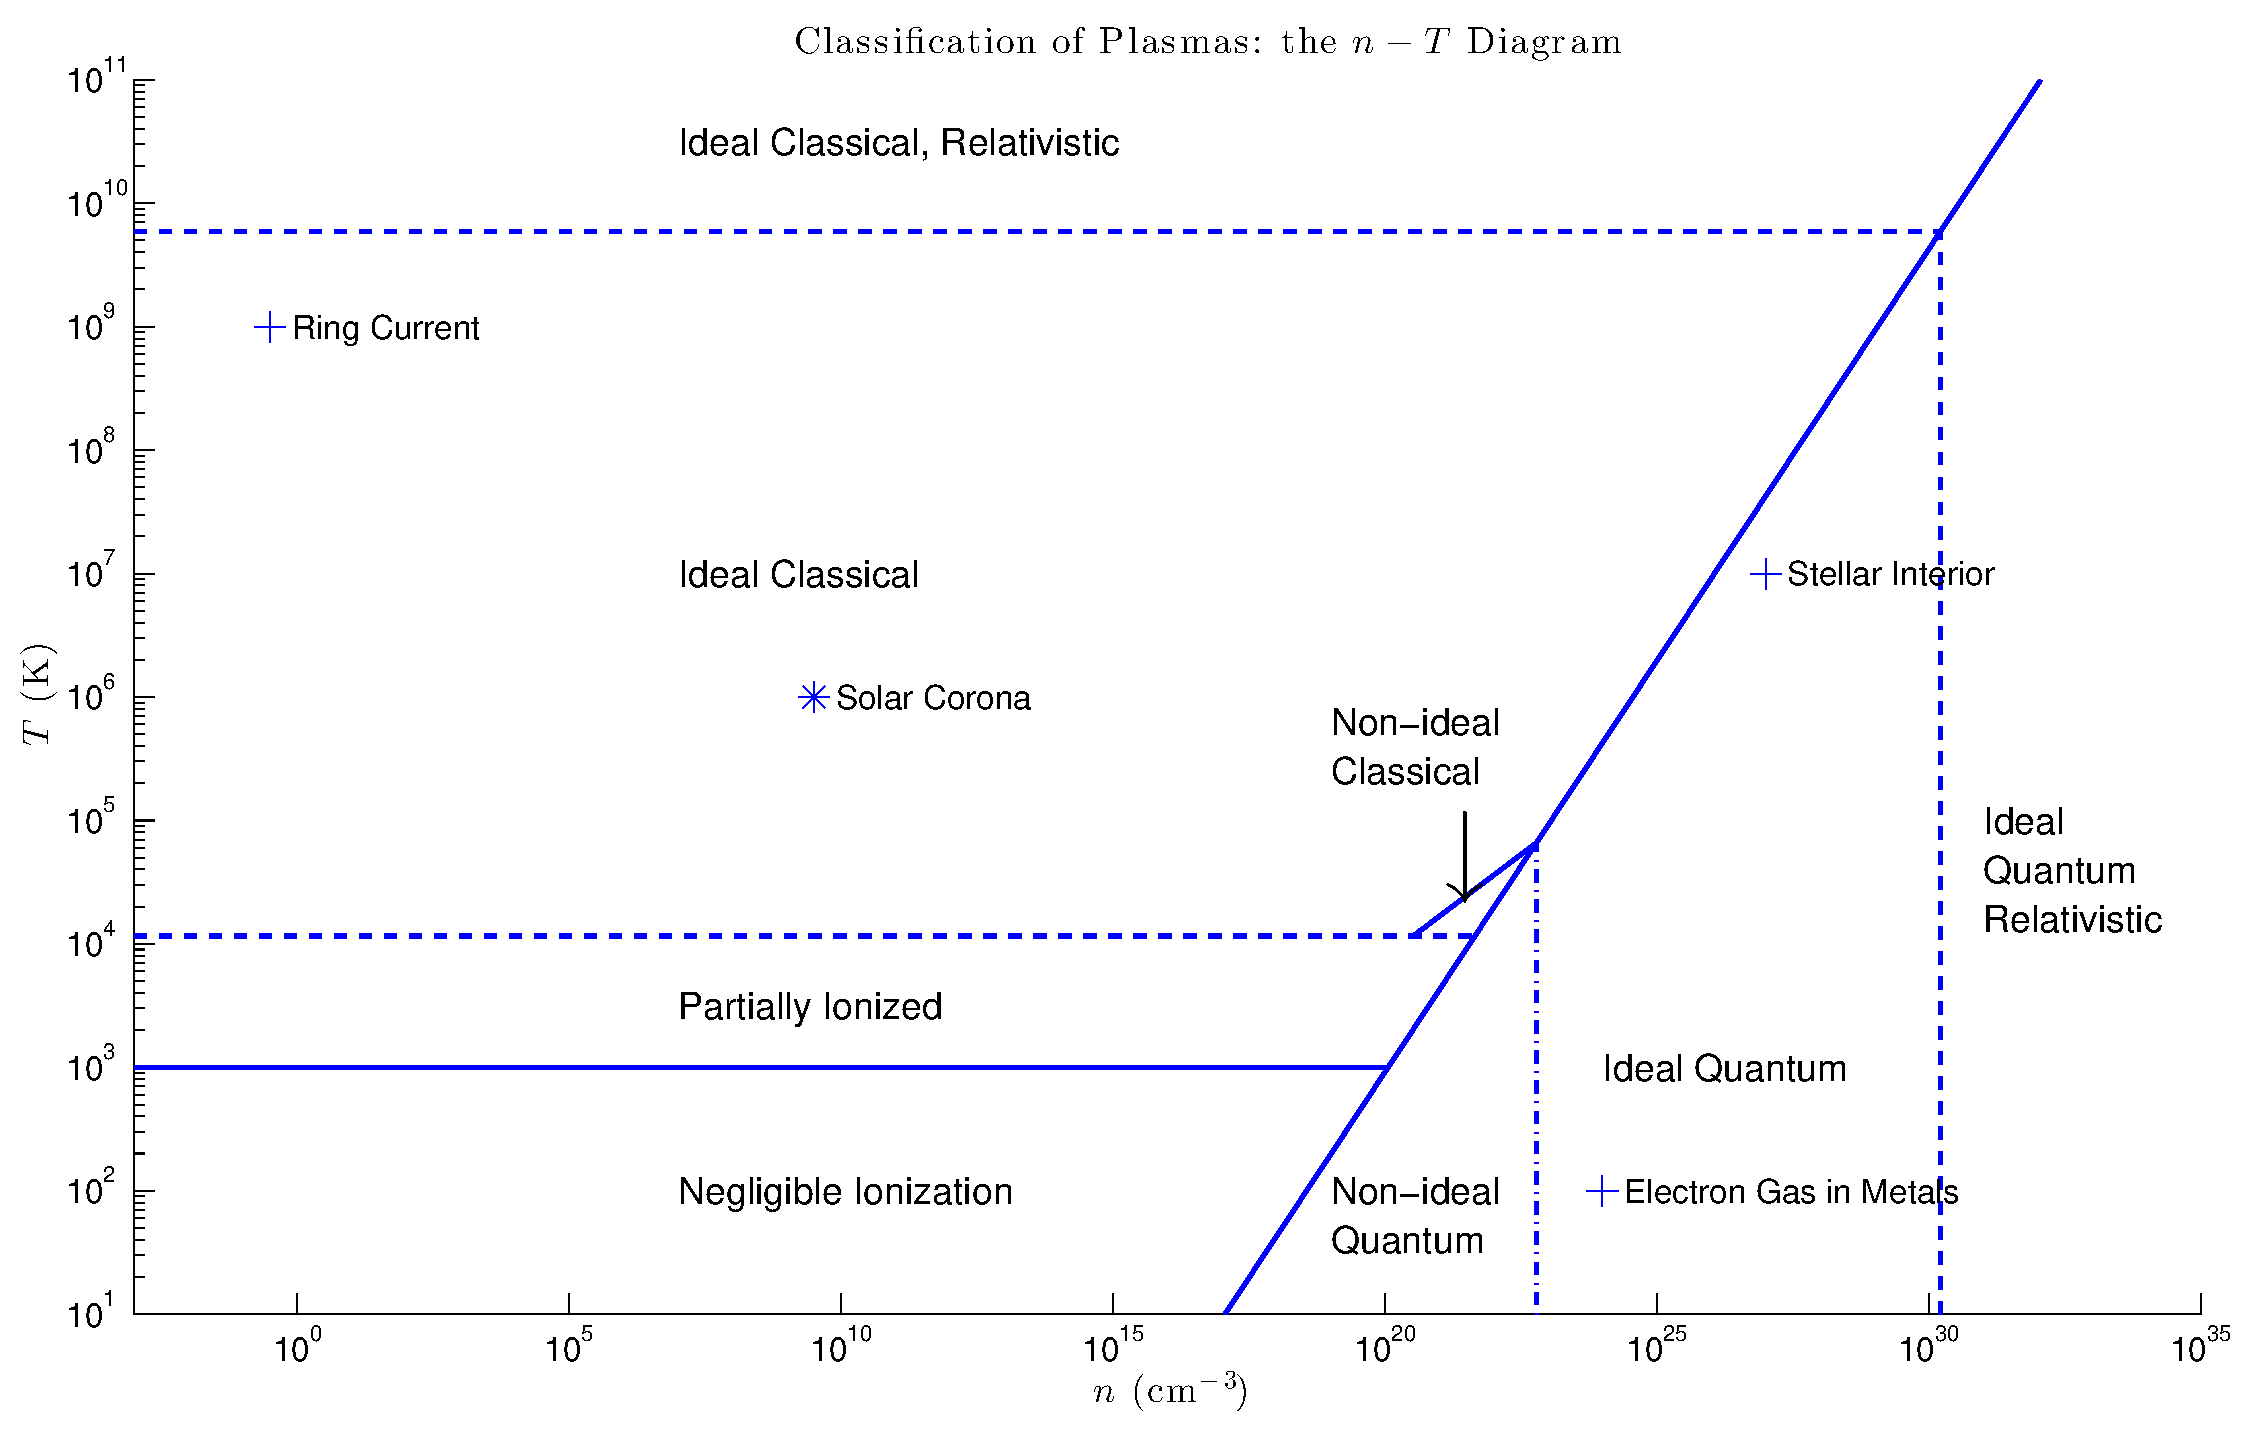
\includegraphics[width=0.7\textwidth]{figures/nT_diagram.eps}
\caption{Phase space diagram for range of density and temperatures with typical plasmas labeled. Plasma is classical (i.e. not quantum) if the average interparticle spacing is much greater than the de Broglie wavelength, $n^{-1/3}\gg h/p$. Alternatively and equivalently, the plasma is classical if the thermal energy is much greater than the Fermi energy, $k_BT\gg E_F=\hbar^2/(3\pi^2n)^{2/3}/(2m_e)$. Weakly-coupled means the average Coulomb interaction energy between two particles is much less than the average kinetic energy, $e^2/n^{-1/3}\ll k_BT$ (classical), $e^2/n^{-1/3}\ll E_F$ (quantum). Similarly, the plasma is non-relativistic provided $T\ll mc^2$ (classical), $E_F\ll mc^2$ (quantum). }
\end{figure}

\section{General Description of a Plasma} 

\newthought{Any statistical system} of mobile charged particles. By ``statistical,'' we mean $N\gg1$; mobile, meaning the particles must be free to move (not trapped in atoms) and because they are charged, they respond to electromagnetic forces. These long-range (i.e. $r^{-2}$) forces are what give rise to \textit{collective behavior} (i.e. every particle interacts with many particles simultaneously).

%
\section{Plasma Characteristics}

	\subsection{Plasma frequency}
	\begin{figure}
		\centering
		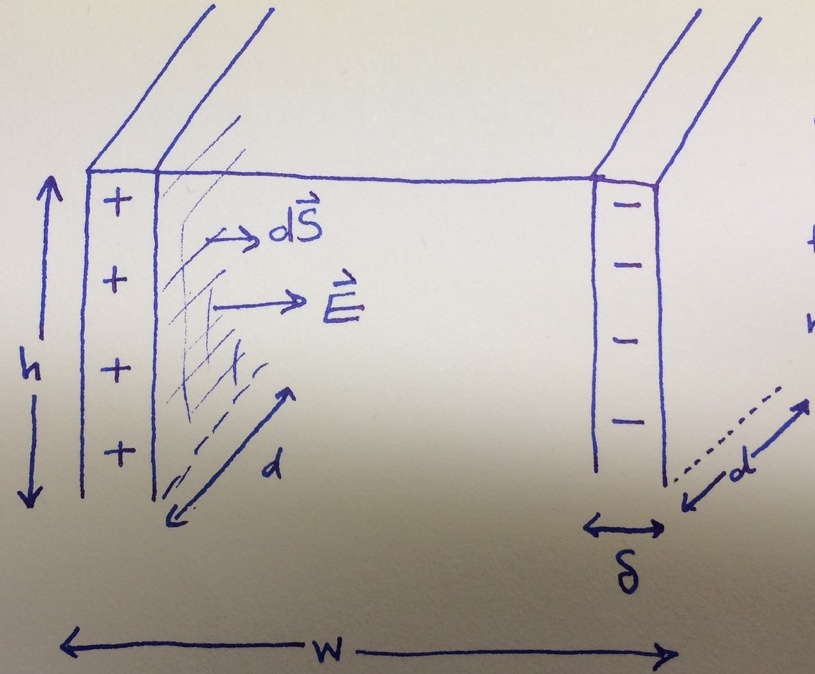
\includegraphics[width=0.4\textwidth]{figures/plasma_frequency.jpeg}
		\caption{Illustration of displaced electrons in uniform block of plasma of width $w$, depth $d$, and height $h$ displaced by an amount $\delta\ll w$.}
		\label{fig:plasma_freq}
	\end{figure}
	Consider the setup in Fig. \ref{fig:plasma_freq}. The block of plasma is quasi-neutral such that $n_e=n_i=n$. The electrons are displaced to the right by $\delta$ such that a slab of positive charge builds up on the left and negative charge on the right. We know that the force on the displaced block is $F=Ma=Q_{tot}E$, where $Q_{tot}=(-e)n(whd)$ and $M=m_en(whd)$. From the integral form of Gauss's law, $\oint\mathrm{d}\vec{S}\cdot\vec{E}=Q_{enc}/\epsilon_0$, we can calculate the electric field due to the $(+)$ slab as $E(dh)=(en(\delta dh))/\epsilon_0~\rightarrow~E=en\delta/\epsilon_0$. Plugging all of this into the equation of motion and noting that $a=\ddot{\delta}$, we get
	\begin{equation}
		\ddot{\delta} + \frac{ne^2}{m_e\epsilon_0}\delta = 0.
	\end{equation}
	Thus, the solutions to this equation are oscillatory with frequency given by,
	\begin{empheq}[box=\widefbox]{align}
		\omega_{pe}^2=\frac{ne^2}{\epsilon_0m_e}~~\text{(SI)},\\
		\omega_{pe}^2=\frac{4\pi ne^2}{m_e}~~\text{(cgs)}.
	\end{empheq}

	\subsection{Debye length}
	Imagine dropping in a positive charge $Q$ into a neutral plasma. $Q$ will attract a cloud of electrons and repel the local ions. Inside the cloud, thermal motions of the electrons will not allow them to escape the electrostatic potential well of $Q$. At the edge of the cloud, the electrostatic potential is shallow enough to allow some of the electrons to escape through thermal motion. The Debye length, defined as,
	\begin{empheq}[box=\widefbox]{align}
		\lambda_D^2 \equiv \frac{\epsilon_0k_BT}{ne^2}~~\text{(SI)},\\
		\lambda_D^2 \equiv \frac{k_BT}{4\pi ne^2}~~\text{(cgs)},
	\end{empheq}
	is a measure of the range of the effect of the test charge $Q$. Note that this range will be greater for a hot, diffuse plasma than for a cold, dense plasma: if $T$ is large, more electrons in the cloud at a given distance from $Q$ will be able to escape the electrostatic potential well so $Q$ is \textit{less} efficiently screened; if the density is lower, electrons will have to be drawn from a larger volume in order to effectively screen $Q$ \citep{dendy_plasma_1990}.

	Also note that the plasma parameter, defined as the number of particles in a Debye cube, is given by
	\begin{equation}
		\Lambda = n\lambda_D^3,
	\end{equation}		
	where $\Lambda\gg1$ (i.e. many particles in the Debye cube) is equivalent to the ``weak-coupling'' condition since it implies that the average interparticle spacing is much less than a Debye length.

	A good way to remember how the different length scales compare to each other is to consider the relation,
	\begin{equation}
		p_0:n_0^{-1/3}:\lambda_D:\lambda_L = \Lambda^{-2/3}:1:\Lambda^{1/3}:\Lambda^{4/3},
	\end{equation}
	where $p_0$ is the distance of closest approach, $n_0^{-1/3}$ is the average interparticle spacing, $\lambda_D$ is the Debye length, and $\lambda_L$ is the mean free path. This is consistent with our previous discussion as we see that when $\Lambda\gg1$, the interparticle spacing is much smaller than the Debye length.

	\subsection{Coulomb collision frequencies}
	\begin{figure}
		\centering
		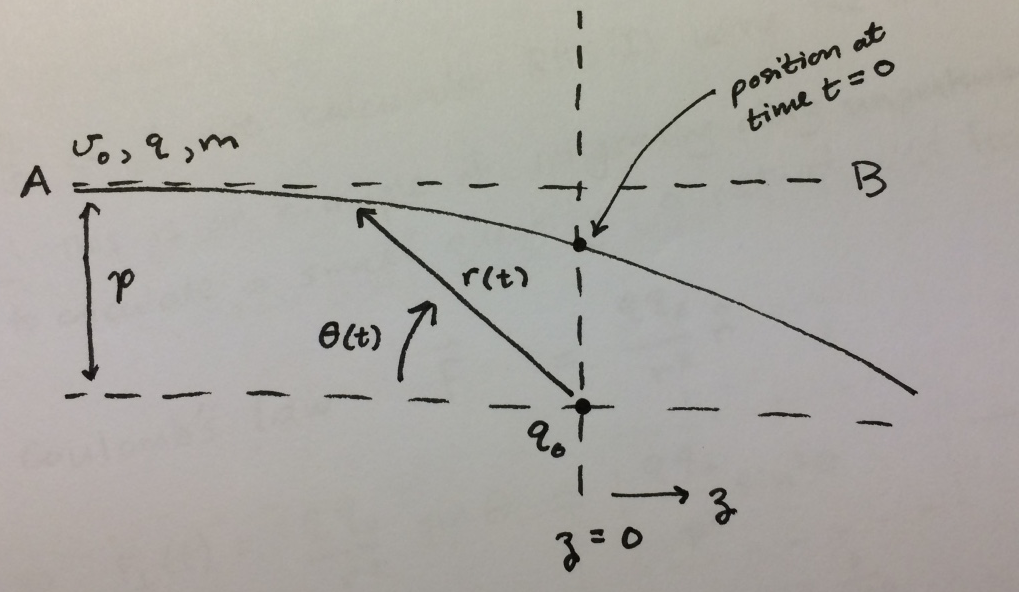
\includegraphics[width=0.6\textwidth]{figures/collisions.png}
		\caption{Collisional cross-section for an incoming test particle of charge $q$ and target particle $q_0$. $p$ is the impact parameter and $v_0$ is the velocity in the horizontal direction.}
		\label{fig:collisions}
	\end{figure}

	Consider an incoming particle with charge $q$ and speed $v_0$ incident on a target $q_0$. When the KE of the test particle is equal to the elecstrostatic potential between $q$ and $q_0$, the test particle will no longer be able to approach the target any closer. In other words, $(1/2)mv_0^2=qq_0/p_0~\rightarrow~p_0=2qq_0/mv_0^2$, where $p_0$ is the distance of closest approach.

	For large-angle collisions (LAC), the collision frequency is given by 
	\begin{equation}
		\label{eq:lac_freq}
		\nu_L=\frac{4\pi n_0e^4}{m_e^2v_0^3}.
	\end{equation}
	The justification is as follows. In a time interval $\delta t$, a test particle traveling at speed $v$ with scattering cross-section $\sigma_L=\pi p_0^2$ will encounter $\delta N=n\sigma v\delta t$ particles. Defining the collision rate or frequency as $\nu_L=\delta N/\delta t$ gives Eq. \ref{eq:lac_freq}. Note that letting $v_0\propto T_e^{1/2}$ implies that as $T_e$ increases, $\nu_L$ decreases. This is because the cross-section decreases with increasing $T_e$ and is the opposite of hard-sphere scattering (i.e. $\nu_{hs}\propto v$).

	Now consider many small-angle collisions (SAC) such that for each, $v_{\perp}\ll v_0$, implying that $p\gg p_0$. Each SAC produces a small change in velocity such that the particle can be thought of as undergoing a random walk in velocity space as it moves through the plasma. From the theory of random walks, we know that $\langle(\Delta v_{\perp,tot})^2\rangle=N\langle(v_{\perp})^2\rangle$. The collision rate can be related to the rate of velocity dispersion by 
	\begin{equation}
		\frac{\mathrm{d}}{\mathrm{d}t}\langle(\Delta v_{\perp,tot})^2 \rangle \equiv \nu_Cv_0^2. 
	\end{equation}
	The LHS can be evaluated by noting that the time-dependence lies in $N$ and as in the LAC case, $\mathrm{d}N/\mathrm{d}t=n_0v_0\mathrm{d}\sigma$ where $\mathrm{d}\sigma=\pi((p+\mathrm{d}p)^2 - p^2)\approx2\pi p\mathrm{d}p$. Plugging all of this in and integrating over the impact parameter $\mathrm{d}p$ gives the formula
	\begin{equation}
		\nu_C=\frac{8\pi n_0e^4}{m_e^2v_0^3}\int^{p_{max}}_{p_{min}}\frac{\mathrm{d}p}{p}.
	\end{equation}
	Because of Debye shielding, the Coulomb force is negligible beyond $\lambda_D$. Thus, $p_{max}\approx\lambda_D$. Additionally, because our approach is not valid beyond $p_0$, $p_{min}\approx p_0$. Using this and noting that $\lambda_D/p_0=\Lambda$, the SAC collision frequency can be written as 
	\begin{empheq}[box=\widefbox]{align}
		\label{eq:sac_freq}
		\nu_C=\frac{8\pi n_0e^4}{m_e^2v_0^3}\ln{\Lambda},
	\end{empheq}
	where $\ln{\Lambda}$ is often referred to as the \textit{Coulomb logarithm}. Note that $\nu_C$ is greater than $\nu_L$ by a factor of $2\ln{\Lambda}$, meaning that for a weakly-coupled plasma, deflection of a particle is primarily due to small-angle collisions rather than large-angle collisions. 

	A few notes on equilibration timescales. First note that $\nu_C/\omega_p=\ln{\Lambda}/2\pi\Lambda$. Suppose, we create an electron-ion plasma with the particles having random positiions and velocities at $t=0$. (1) On a timescale $\sim2\pi/\omega_p$, Debye shielding clouds are set up; (2) on a time scale $1/\nu_{ei}\sim1/\nu_{ee}$ ($\sim2\pi\Lambda/\ln{\Lambda}$ longer than (1)) electrons thermalize by collisions with other electrons and ions; (3) on a timescale $1/\nu_{ii}\sim\sqrt{m_i/m_e}1/\nu_{ei}$, the ions thermalize; and (4) on a timescale $1/\nu_{ie}\sim\sqrt{m_i/m_e}1/\nu_{ii}$, the ions and electrons thermalize to the same temperature. 

	\subsection{Spitzer resistivity}
	By ``Spitzer'' resistivity, we simply mean resistivity due to collisions. From Ohm's law, we know that $\mathbf{E}=\eta\mathbf{j}$. Using $\mathbf{j}=en\mathbf{v}$, and plugging this into a generalized equation of motion,
	\begin{equation}
		m\frac{\partial \mathbf{v}}{\partial t} = \eta e^2n\mathbf{v}.
	\end{equation}
	We can estimate the RHS as $\approx m\mathbf{v}/\tau$, where $\tau=1/\nu_{ei}$ is a characteristic diffusion time. Thus, we can solve for the resistivity, using $v_0\approx v_{th}=\sqrt{k_BT/m_e}$,
	\begin{equation}
		\eta=8\pi e^2\sqrt{\frac{m_e}{(k_BT)^3}}\ln{\Lambda}.
	\end{equation}

\section{Particle Motion in Electric \& Magnetic Fields}

	\subsection{Drifts}

	\newthought{The Larmor radius, $\rho$,} can be derived by setting $|\mathbf{F}_B|=|\mathbf{F}_C|~\rightarrow~qv_{\perp}B=mv_{\perp}^2/\rho~\rightarrow~\rho=v_{\perp}/\omega_C$ where $\omega_C=qB/m$ is the cyclotron frequency. For charged particle motion in a uniform static magnetic field such that $\mathbf{B}=B\hat{z}$, the equation of motion $m\dot{\mathbf{v}}=q(\mathbf{v}\times\mathbf{B})$, can be written component-wise as
	\begin{align}
		\dot{v}_z &= 0 \\[0.5em]
		\dot{v}_x &= \omega_Cv_y \\[0.5em]
		\dot{v}_y &= -\omega_Cv_x.
	\end{align}
	Using a little bit of algebra, the formulas for $x(t),y(t),z(t)$ can be found
	\begin{align}
		x &= x_0 + \frac{v_{\perp}}{\omega_C}\sin{\omega_Ct+\phi_0} \\[0.5em]
		y &= y_0 + \frac{v_{\perp}}{\omega_C}\cos{\omega_Ct+\phi_0} \\[0.5em]
		z &= z_0 + v_zt,
	\end{align}
	such that the motion is \textit{helical} with radius $\rho$, the Larmor radius. Thus, the ``guiding center'' (GC) has coordinates $(x_0,y_0,z)$ (i.e. center of gyration translates along $z-$axis.)

	\begin{enumerate}

		\item{GC Drift due to Non-magnetic Forces} 
		Consider the configuration shown in Fig. \ref{fig:gyroradius} such that the particle position is $\mathbf{x}=\mathbf{X}+\mathbf{\rho}$ where $\mathbf{\rho}\equiv(1/\omega_c)\hat{\mathbf{b}}\times\mathbf{v}$ where $\hat{\mathbf{b}}\equiv\mathbf{B}/B$ is the gyroradius vector and $\mathbf{X}$ is the guiding center. Consider the equation of motion $m\dot{\mathbf{v}} = q\mathbf{v}\times\mathbf{B}+\mathbf{F}$, where $\mathbf{F}$ is some static, uniform force.

		Differentiating $\mathbf{X},\dot{\mathbf{X}}=\mathbf{v} - \hat{\mathbf{b}}\times\dot{\mathbf{v}}/\omega_c$ and using the EOM yields 
		\begin{equation}
			\dot{\mathbf{X}}= v_{\parallel}\hat{\mathbf{b}} + \frac{1}{qB}\mathbf{F}\times\mathbf{B},
		\end{equation}
		where the first term is parallel to $\mathbf{B}$ and the second term is called the guiding center drift velocity
		\begin{empheq}[box=\widefbox]{align}
			\label{eq:gc_drift}
			\mathbf{V}_d \equiv \frac{1}{qB^2}\mathbf{F}\times\mathbf{B}.
		\end{empheq}
		If $\mathbf{F} = q\mathbf{E}$, where $\mathbf{E}$ is the electric field, then Eq. \ref{eq:gc_drift} becomes $\mathbf{V}_d = \mathbf{E}\times\mathbf{B}/B^2$, the ``E-cross-B'' drift velocity. Note that it is independent of charge so electrons and ions drift in the same direction.
		\begin{figure}
			\centering
			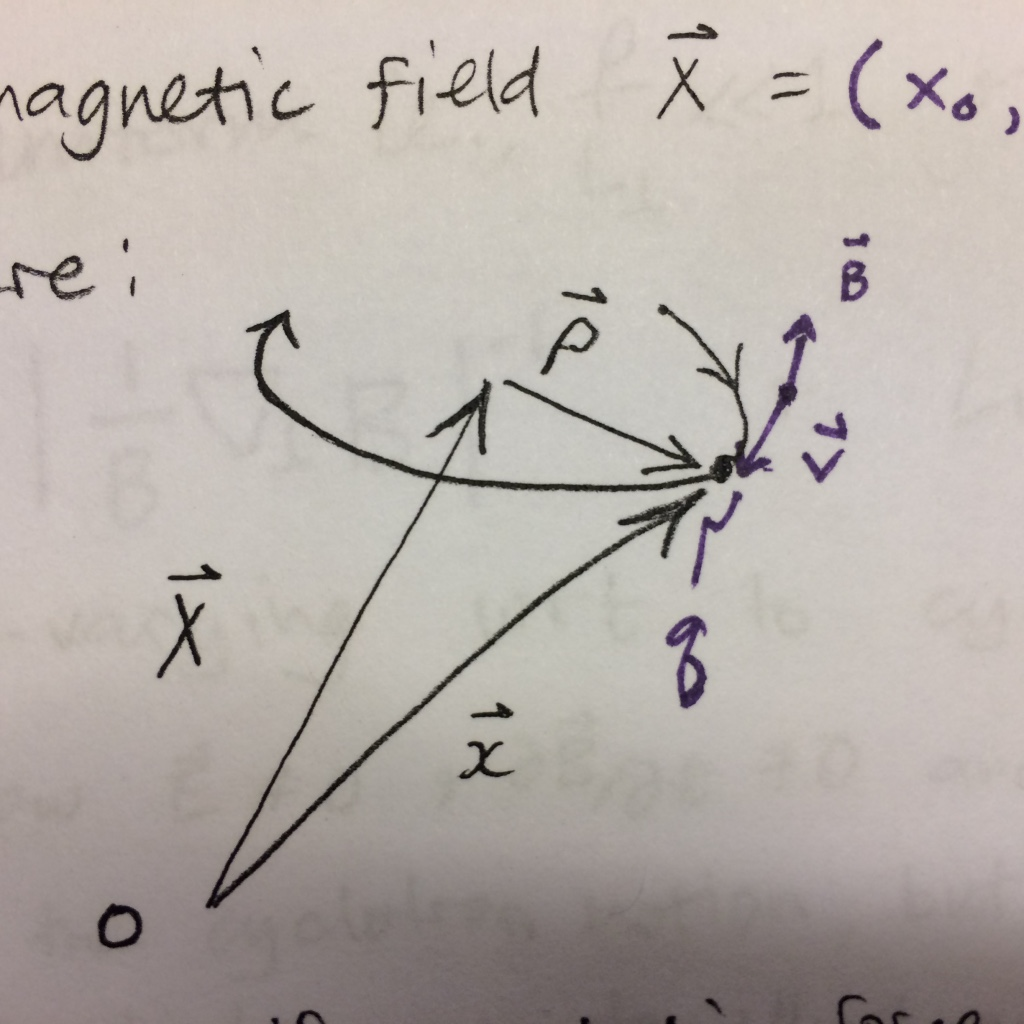
\includegraphics[width=0.5\textwidth]{figures/gyroradius_schematic.jpeg}
			\caption{Schematic showing particle position $\mathbf{x}$ in terms of the guiding center position $\mathbf{X}$ and the Larmor radius $\mathbf{\rho}$}
			\label{fig:gyroradius}
		\end{figure}

		\item{GC Motion in a Nonuniform Magnetic Field} 
		Consider a weakly non-uniform field such that the B-field changes very little over one cyclotron orbit. The perpendicular guiding center velocity is given by
		\begin{equation}
			\label{eq:more_drifts}
			\mathbf{v}_{\perp} = \frac{\mu}{qB}\hat{b}\times\nabla B +  \frac{v_{\parallel}^2}{\omega_c}\hat{b}\times \frac{\partial \hat{b}}{\partial s},
		\end{equation}
		where $\mu=mv_{\perp}^2/2B$, the first term is the $\nabla B$ drift, $\mathbf{v}_{\nabla}$ and the second term is the curvature drift, $\mathbf{v}_C$. An example of $\nabla B$ drift is \textit{magnetic mirroring}. Using $\nabla\cdot\mathbf{B}=0$ and $\partial B_z/\partial z,\partial B_r/\partial r\neq0$, it can be shown that $F_z=-\mu\partial B_z/\partial z$ such that as the field strength grows in the $+z-$direction, the force in the $-z-$direction increases. If this gradient in $z$ is symmetric (as in the dipole field of the Earth), the particle can become trapped.

		Note that this kind of drift motion, as well as the drift due to non-magnetic forces, occured because the particle spiraling around the field sampled the magnetic field inhomogeneity. We now consider curvature drift due to the curvature of magnetic field lines. Suppose there is a non-inertial frame that follows the particle along its curved path and in this frame, the position is described by position $\mathbf{r}$. The position of the particle in the inertial frame is $\mathbf{R}$ such that $\mathbf{c}=\mathbf{R}-\mathbf{r}$ is the position of the non-inertial frame in the inertial frame. Because the particle is curving (in the inertial frame), it is subject to a centripetal force $\mathbf{F}=m\ddot{\mathbf{R}}$.

		Thus, the force in the non-inertial frame can be written as $m\ddot{\mathbf{r}}=\mathbf{F} - m\ddot{\mathbf{c}}$. Defining $\mathbf{F}_c=-m\ddot{\mathbf{c}}$, we note that $\mathbf{F}_c$ is the force resulting from the fact that the comoving frame is non-inertial. Thus, $\ddot{\mathbf{c}}=v_{\parallel}^2\mathbf{R}_C$, where $\mathbf{R}_C=\partial\hat{b}/\partial s$ is the local radius of curvature, where $s$ denotes the field-aligned coordinate. Plugging this into Eq. \ref{eq:gc_drift}, we get the second term in Eq. \ref{eq:more_drifts}.

	\end{enumerate}
	
	\subsection{Adiabatic invariants}

	The first adiabatic invariant is the magnetic moment $\mu$ as given by $\mu=mv_{\perp}^2/2B$. The constancy of $\mu$ is equivalent to saying the magnetic flux through the particle orbit is conserved. Note also that the invariance of $\mu$ depends on the slow variation of $\mathbf{B}$ over a single cyclotron orbit. Thus, this first adiabatic invariant is associated 

	The second adiabatic invariant can be written as 
	\begin{equation}
		J_b\equiv\oint\mathrm{d}s~p_{\parallel},
	\end{equation}
	where the integral is taken along the bouncing guiding center trajectory. $J_b$ is an adiabatic invariant provided that the field changes slowly over a single bounce period. Thus, this second adiabatic invariant is associated with the periodic bounce motion.

	The third adiabatic invariant can be written as 
	\begin{equation}
		\psi\equiv\int_d\mathrm{d}\mathbf{s}\cdot\mathbf{B},
	\end{equation}
	where the integral is taken over a surface whose edge is defined by the bounce center drift. The bounce center drifts perpendicular to $\mathbf{B}$ by $\nabla B$ and curvature drifts, giving a third periodic motion. $\psi$ is an adiabatic invariant provided the field changes slowly compared to the bounce center drift period.

\section{Waves in Plasma}

\newthought{First,} consider the general formulation for the calculation of wave modes in a cold plasma. Combining Eq. \ref{eq:faraday} with $\partial/\partial t$ of Eq. \ref{eq:ampere_maxwell} and using well-known vector identities, we note that 
\begin{equation}
	\label{eq:dispersion_maxwell}
	\nabla^2\mathbf{E} - \nabla(\nabla\cdot\mathbf{E}) = \frac{1}{c^2}\left(4\pi\frac{\partial\mathbf{j}}{\partial t} + \frac{\partial^2\mathbf{E}}{\partial t^2}\right).
\end{equation}
Next, we recall that the generalized Ohm's law is written as $\mathbf{J}=\tensor{\sigma}\cdot\mathbf{E}$ such that $\partial\mathbf{j}/\partial t=\tensor{\sigma}\cdot\partial\mathbf{E}/\partial t$. For monochramtic plane-wave solution, the electric field can be written as $\delta\mathbf{E}=\delta\mathbf{E}_0\exp{(i\mathbf{k}\cdot\mathbf{x}-i\omega t)}$ such that $\partial/\partial t\to-i\omega$ and $\nabla\to i\mathbf{k}$. Thus, the RHS of Eq. \ref{eq:dispersion_maxwell} becomes
\begin{equation}
\frac{1}{c^2}\left(4\pi\tensor{\sigma}\cdot\frac{\partial\mathbf{E}}{\partial t} + \frac{\partial^2\mathbf{E}}{\partial t^2}\right) = \frac{1}{c^2}\left(-4\pi i\omega\tensor{\sigma}\cdot\mathbf{E} - \omega^2\mathbf{E}\right) = -\frac{\omega^2}{c^2}\left(\frac{4\pi i}{\omega}\tensor{\sigma} + \mathbb{I}\right)\mathbf{E}.
\end{equation}
Furthermore, we can define the dielectric tensor as $\tensor{\varepsilon}=\mathbb{I} + (4\pi i/\omega)\tensor{\sigma}$. Using this and our plane wave solutions, we can rewrite Eq. \ref{eq:dispersion_maxwell} as
\begin{equation}
-k^2\mathbf{E} + \mathbf{k}(\mathbf{k}\cdot\mathbf{E}) + \frac{\omega^2}{c^2}\tensor{\varepsilon}\cdot\mathbf{E} = 0.
\end{equation}
Defining the disperson tensor as $\tensor{\mathcal{D}}=-k^2\mathbb{I} + \mathbf{kk} + (\omega^2/c^2)\tensor{\varepsilon}$,  Eq. \ref{eq:dispersion_maxwell} can be written as $\tensor{\mathcal{D}}\cdot\mathbf{E}=0$ which has non-trivial solutions if and only if $\|\tensor{\mathcal{D}}\|=0$. This is the dispersion relation. In general, for given $\mathbf{k}$, it will have $n$ solutions $\omega_n(k)$. These $\omega_n$ are called the \textit{normal modes} of the plasma.

	\subsection{Cold unmagnetized plasma}

	We note that ``cold'' means negligible thermal motion (i.e. ``zero temperature'') and unmagnetized means no background magnetic field. Given the assumption of a one-component electron plasma of density $n_0$, for plane-wave solutions of the velocity and electric field, the equation of motion can be written as $m_e\delta\dot{\mathbf{v}}=-e\delta\mathbf{E}$. Solving this equation yields $\delta\mathbf{v}=(e/i\omega m_e)\delta\mathbf{E}$. Using the generalized Ohm's law and noting that the current density can be written as $\delta\mathbf{j}=-en_0\delta\mathbf{v}$, the conductivity tensor for a cold, unmagnetized one-component plasma can be written as
	\begin{equation}
		\tensor{\sigma} = \frac{in_0e^2}{\omega m_e}\mathbb{I}
	\end{equation}
	and thus the dielectric tensor is $\tensor{\varepsilon} = (1-(\omega_{pe}/\omega)^2)\mathbb{I}$. Using these relations, we can now write the dispersion tensor as $\tensor{\mathcal{D}} = ((\omega^2 - \omega_{pe}^2)/c^2 - k^2)\mathbb{I} + \mathbf{kk}$. Without loss of generality, we choose $\mathbf{k}=k\hat{z}$ such that $\tensor{\mathcal{D}}$ can be written as
	\begin{equation}
		\label{eq:dt_um}
		\tensor{\mathcal{D}} = 
		\begin{bmatrix}
			\mathcal{D}_T & 0 & 0\\
			0 & \mathcal{D}_T & 0\\
			0 & 0 & \mathcal{D}_L\\
		\end{bmatrix}
		,
	\end{equation}
	where $\mathcal{D}_T\equiv((\omega^2 - \omega_{pe}^2)/c^2 - k^2)$ and $\mathcal{D}_L\equiv(\omega^2 - \omega_{pe}^2)/c^2$. The dispersion relation can then be expressed as, $\|\tensor{\mathcal{D}}\| = 0\rightarrow\mathcal{D}_T^2\mathcal{D}_L=0$. We now find the normal modes for the cases of $\mathcal{D}_T=0$ and $\mathcal{D}_L=0$.

	For $\mathcal{D}_T=0$,  $\omega^2=\omega_{pe}^2 + k^2c^2$. Note that in the limit of no plasma ($n_0=0$), this reduces to $\omega=kc$, the vacuum plane-wave solutions. $\mathcal{D}_T=0$ implies that Eq. \ref{eq:dt_um} reduces to $\mathcal{D}_L\delta E_z=0$. Because $\mathcal{D}_L\neq0$, $\delta E_z=0$ with $\delta E_x,\delta E_y\neq0$. Recalling that $\mathbf{k}=k\hat{z}$, it follows that $\mathbf{k}\perp\delta\mathbf{E}$. Thus, these wave solutions are \textit{transverse electromagnetic waves}.

	For $\mathcal{D}_L=0$, $\omega^2=\omega_{pe}^2$, plasma oscillations at the plasma frequency $\omega_{pe}$. $\mathcal{D}_L=0$ implies that $\mathcal{D}_T\delta E_x=0$ and $\mathcal{D}_T\delta E_y=0$. Since $\mathcal{D}_T\neq0,$ we have that $\delta E_x,\delta E_y=0$ and $\delta E_z\neq0$. Thus, $\mathbf{k}\parallel\mathbf{E}$ and these wave solutions are \textit{longitudinal electrostatic waves}.

	\subsection{Cold magnetized plasma}

	Now suppose the background plasma has a uniform magnetic field $\mathbf{B}_0=B_0\hat{z}$. Using Fourier amplitudes and dropping second order terms, the equation of motion can thus be written as 
	\begin{eqnarray}
		\label{eq:cmp_eom}
		m_e\delta\dot{\mathbf{v}} &=& -e(\delta\mathbf{E} + \delta\mathbf{v}\times(\mathbf{B}_0+\delta\mathbf{B})), \\ 
		m_e\delta\dot{\mathbf{v}} &\approx& -e(\delta\mathbf{E} + \delta\mathbf{v}\times\mathbf{B}_0), \\
		(-i\omega - \mathbf{\Omega}\times)\delta\mathbf{v} &=& -\frac{e}{m_e}\delta\mathbf{E},
	\end{eqnarray}
	where $\mathbf{\Omega}\equiv (eB_0/m_e)\hat{z}=\omega_{ce}\hat{z}$. By applying the conjugate operator $(i\omega-\mathbf{\Omega})$ and noting that $\mathbf{J}=-en_0\mathbf{v}=\tensor{\sigma}\cdot\mathbf{E}$, we can solve for both $\tensor{\sigma}$ and $\tensor{\varepsilon}$. 

	To define a more general dielectric tensor for a multispecies plasma, we consider a current density $\delta\mathbf{j}=\sum_sq_sn_{s0}\delta\mathbf{v}_s$, where $s$ is the species label such that there are $s$ EOMs $m_s\delta\dot{\mathbf{v}}_s = q_s\delta\mathbf{E} + q_s\delta\mathbf{v}_s\times \mathbf{B}_0$. The resulting dielectric tensor is,
	\begin{equation}
		\tensor{\varepsilon} = 
		\begin{bmatrix}
			S & -iD & 0\\
			iD & S & 0\\
			0 & 0 & P
		\end{bmatrix}
		,
	\end{equation}
	where
	\begin{align}
		S,D \equiv \frac{1}{2}(R\pm L),\label{eq:sd_mode}\\
		R,L \equiv 1 - \sum_s\frac{\omega_{ps}^2}{\omega}\frac{1}{\omega\pm\omega_{cs}},\label{eq:rl_mode}\\
		P \equiv 1 - \sum_s\frac{\omega_{ps}^2}{\omega^2}.\label{eq:p_mode}
	\end{align}
	Using $\mathbf{n}= c\mathbf{k}/\omega$, the dispersion tensor can be written as $\tensor{\mathcal{D}}=(\omega^2/c^2)(\tensor{\varepsilon} + \mathbf{nn} - n^2\mathbb{I})$. Thus, choosing, without loss of generality, $\mathbf{k}=(k_x,0,k_z)$, $\tensor{\mathcal{D}}$ for a cold, unmagnetized, multi-component plasma can be written as
	\begin{equation}
		\label{eq:dt_mp}
		\tensor{\mathcal{D}} = 
		\begin{bmatrix}
			S - n_z^2 & -iD & n_xn_z \\ 
			iD & S-n^2 & 0 \\
			n_xn_z & 0 & P-n_x^2
		\end{bmatrix}
		.
	\end{equation}

	We now want to find the disperson relation $\|\tensor{\mathcal{D}}\|=0$. Noting that $n_x=n\sin{\theta},~n_z=n\cos{\theta}$, and defining $A=S\sin^2\theta+P\cos^2\theta,~B=RL\sin^2\theta+PS(1+\cos^2\theta),$ and $C=PRL$, the ``Stix'' form of the dispersion relation can be written as
	\begin{equation}
		\label{eq:stix_dr}
		An^4 - Bn^2 + C =0,
	\end{equation}
	implying that there are zero, one, or two real roots to the dispersion relation. Equivalently, after some algebra, the ``Astrom-Allis'' form of the dispersion relation can be written
	\begin{equation}
		\label{eq:aa_dr}
		\tan^2\theta = \frac{-P(n^2-R)(n^2-L)}{(Sn^2 - RL)(n^2 - P)}.
	\end{equation}

	Two quick notes on normal modes in a cold magnetized plasma:(1) $\omega_{pi}^2/\omega_{pe}^2\sim m_e/m_i\sim10^{-3}$, $\omega_{ci}^2/\omega_{ce}^2\sim(m_e/m_i)^2\sim10^{-6}$, and for many fusion and space plasmas, $\omega_{ce}\sim\omega_{pe}$. Thus, we have the following separation of frequency scales,
	\begin{equation}
		\text{``low frequency''}~\omega_{ci}^2\ll\omega_{pi}^2\ll\omega_{ce}^2\sim\omega_{pe}^2~\text{``high frequency''}.
	\end{equation}
	(2) From Eq. \ref{eq:stix_dr}, it can be shown that $n=kc/\omega$ must be either purely real ($n^2>0$, propagating) or purely imaginary ($n^2<0$, evanescent). Thus, our model does not allow for $n\in\mathbb{C}$ (i.e. damping or instabilities) as our treatment is too simple to include such effects.

	We now consider several different wave modes that can arise in a cold, magnetized, electron-ion plasma. We will use Eq. \ref{eq:aa_dr} for two different values of $\theta$.

	\begin{itemize}
		\item{$\theta=0$, parallel propagation}
		\begin{figure}
			\centering
			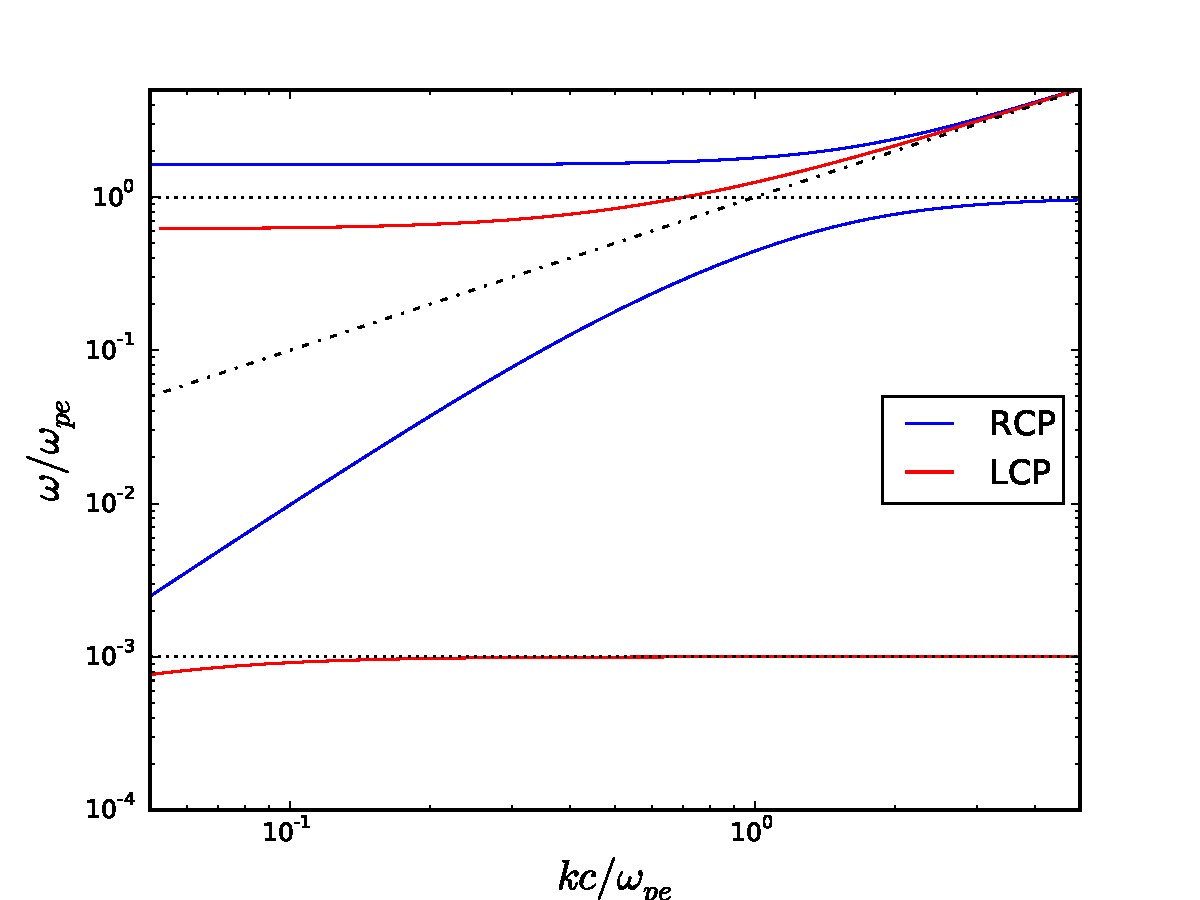
\includegraphics[width=0.6\textwidth]{figures/cmp_dispersion.pdf}
			\caption{Dispersion curves for R- and L-waves for parallel propagation. The dotted line at $y=x$ represents $\omega=kc$. The lower dotted lines are $\omega_{ce}$ and $\omega_{ci}$, respectively.}
		\end{figure}

		LHS of Eq. \ref{eq:aa_dr} $=0$ which implies $P(n^2 - R)(n^2 - L)=0$. We consider the three possible cases in which the numerator could be zero.

		\begin{enumerate}
			\item{$P=0$}
			From Eq. \ref{eq:p_mode}, we see that $P=0=1-\sum_s\omega_{ps}^2/\omega^2$ which for $s=e,i$ can be rewritten as $\omega^2=\omega_{pe}^2+\omega_{pi}^2$. Recalling that $\omega_{pe}^2/\omega_{pi}^2=m_e/m_i\ll1$, we find that the $P=0$ case implies $\omega^2\approx\omega_{pe}^2$. Note that this is the same dispersion relation as that for electrostatic plasma waves in the unmagnetized plasma. Substituting $P=0$ into the wave equation yields $\mathbf{k}\parallel\delta\mathbf{E}$ and $\delta\mathbf{B}=0$. Thus, these waves are longitudinal electrostatic plasma waves or plasma oscillations. Note that plasma oscillations $\parallel$ to $\mathbf{B}_0$ are not affected by $\mathbf{B}_0$. 
			
			\item{$n^2=R$}
			Looking back to the wave equation $\tensor{\mathcal{D}}\cdot\mathbf{E}=0$ (see Eq. \ref{eq:dt_mp}), for $n^2=R$ (noting $n_x=0,~n_z=n$ for $\theta=0$), we find that $P\delta E_z=0$ and $\delta E_y=i\delta E_x$. This implies that $\delta E_z=0$ (because $P\neq0$ in this case) and $\delta E_x$ and $\delta E_y$ are out of phase by $\pi/2$. Thus, for some given location $z=z_0$ and noting $\mathbf{k}\cdot\mathbf{z}=kz_0$, $\delta E_x=E_0\mathrm{Re}(\exp{(ikz_0-i\omega t)})=E_0\cos{(\omega t-kz_0)}$ and $\delta E_y=E_0\mathrm{Re}(\exp{(ikz_0)}i\exp{(-i\omega t)})=E_0\sin{(\omega t - kz_0)}$. Thus, $\delta\mathbf{E}$ rotates in a right-handed sense with respect to $\mathbf{B}_0=B_0\hat{z}$; so $n^2=R$ corresponds to \textit{right circularly polarized electromagnetic waves}, or RCP EM waves (sometimes just called ``R waves'').
			\par Using the fact that $n^2=k^2c^2/\omega^2$ and Eq. \ref{eq:rl_mode}, we see that $n^2\to\infty$ (or $k\to\infty$ or $\lambda\to0$) as $\omega\to|\omega_{ce}|$ from below. This is an example of an electron cyclotron resonance (ECR); $\delta\mathbf{E}$ rotates in phase with the electron cyclotron motion. In a ``warm'' or ``hot'' plasma, these waves can heat the particles.
			\par Recalling that $n^2>0$ corresponds to propagation while $n^2<0$ implies evanescent waves, $n^2=0$ corresponds to the cutoff (i.e. when waves no longer propagate). Thus, solving for $\omega$ in $n^2=R=0$ yields, assuming $\omega^2\gg\omega_{pi}^2,\omega_{ci}^2$,
			\begin{equation}
				\omega_R\equiv\frac{|\omega_{ce}|}{2}\left(\sqrt{1+\frac{4\omega_{pe}^2}{\omega_{ce}^2}} + 1\right).
			\end{equation}
			This is called the R-wave cutoff frequency, where $\omega_R>\omega_{ce}$. Note that in the high-frequency limit, $\omega^2\gg\omega_{pe}^2,\omega_{ce}^2$ and $\omega=kc$, the vacuum EM wave solution. At lower, but high frequencies, $\omega^2\gtrsim\omega_R^2$. Using the definition of $\omega_R$, we note that $\omega\gtrsim\omega_R$ implies propagation while $\omega\lesssim\omega_R$ implies evanescence. At even lower frequencies, $\omega^2\sim\omega_{ce}^2$, $\omega\to\omega_{ce}$ from above and $n^2\to-\infty$, implying evanescence. Thus, for $\omega_2<\omega_{ce}^2$, $n^2>0$, implying propagation. Finally, we can conclude that an R wave propagates when $\omega>\omega_R$ or $\omega<|\omega_{ce}|$, but not in between. In the frequency range $\omega<|\omega_{ce}|$, the R wave is often called the electron cyclotron wave (ECW). 
			\par An example of an ECW in space physics is the whistler wave, whose signal starts at high frequencies and finishes at low frequencies. Its frequency is in the range $\omega_{pi}^2\ll\omega^2\ll\omega_{ce}^2$. These waves are produced when a lightning strike (an EM pulse) generates an ECW with $\omega<\omega_{ce}$ in the ionosphere which then propagates to the opposite hemisphere. Some of the wave energy is transmitted through the ionosphere to the ground where it may be detected. Using $n^2=R$, the whistler wave dispersion relation can be shown to be $\omega_{Wh}=(|\omega_{ce}|c^2/\omega_{pe}^2)k^2$. Noting that the group velocity, $v_g=\partial\omega/\partial k$, we see that for Whistler waves, $v_g\propto k$ such that high frequency waves will arrive first, explaining the observed high to low tones of whistler waves.

			\item{$n^2=L$}
			This wave is a left circularly polarized (LCP) EM wave such that $\delta\mathbf{E}$ rotates with the same sense as ion cyclotron motion. The ``L wave'' propagates if $\omega<\omega_{ci}$ and has a resonance at $\omega_{ci}$. Furthermore, it does not propagate for $\omega_{ci}<\omega<\omega_L$, where $\omega_L\equiv(|\omega_{ce}|/2)(\sqrt{1+\frac{4\omega_{pe}^2}{\omega_{ce}^2}} - 1)$ is the ``L wave'' cutoff frequency. Note that $\omega_L>|\omega_{ce}|$ when $\omega_{pe}^2>2\omega_{ce}^2$. This wave also propagates in the range $\omega>\omega_L$. Note that the ion cyclotron resonance can be used to heat tokamak plasmas, the casis of ion cyclotron range of frequencies heating (ICRF).

			\item{General Features of parallel waves}
			In the regime $\omega^2\ll\omega_{ci}^2\ll\omega_{ce}^2$, $R\sim L$ and the ECW and ICW merge into a wave called the shear Alfv\'{e}n wave (SAW) with frequency $\omega^2=k_{\parallel}^2V_A^2$ where $V_A\equiv B_0^2/(\mu_0\rho)$ is called the Alfv\'{e}n speed. The SAW is a linearly polarized transverse EM wave  and arguably the most important low-frequency wave in plasma physics. This is because they are easily excited by large-scale perturbations of the plasma and can transport large amounts of energy through the plasma (mostly along field lines).

			Faraday rotation can be understood in the context of a linearly polarized wave written as the sum of an LCP wave and an RCP wave. For $\mathbf{B}_0$, the ECW and ICW propagate at different speeds and so the plane of polarization rotates. The effect can be seen in an angle between the initial orientation before entering the plasma and after traveling some distance $L$ through the plasma. This effect can be used to measure magnetic field strengths in astrophysical contexts if the density is known. 
		\end{enumerate}

		\item{$\theta=\pi/2$, perpendicular propagation}
		LHS of Eq. \ref{eq:aa_dr} $\to\infty$ which implies  $(Sn^2 - RL)(n^2 - P)=0$. We consider the three possible cases in which the denominator could be zero.

		\begin{enumerate}

			\item{$n^2=RL/S$}
			More complicated than ``O waves'' and are commonly referred to as ``X waves'' (or ``extraordinary'' waves). They have both a longitudinal and transverse $\delta\mathbf{E}$ and experience a cutoff at $\omega_R$ and $\omega_L$. Additionally, two resonances can occur: the upper hybrid resonance $\omega_{un}^2=\omega_{pe}^2 + \omega_{ce}^2$ and the lower hybrid resonance $\omega_{lh}^2 = \omega_{ci}|\omega_{ce}|$

			\item{$n^2=P$}
			Using $n=kc/\omega$ and the definition of $P$ from Eq. \ref{eq:p_mode}, the resulting dispersion relation is $\omega^2=k^2c^2 + \omega_{pe}^2$, the same dispersion relation as the ``ordinary'' transverse EM waves in a cold unmagnetized plasma. These are called ``O waves''. They are linearly polarized transverse EM waves with $\delta\mathbf{E}\parallel\mathbf{B}_0$ such that the field has no effect on the wave. 
		\end{enumerate}
	\end{itemize}

	\subsection{More\ldots? See kinetic theory notes}

\section{Magnetohydrodynamic (MHD) Description of Plasma}

The ideal MHD equations are
\begin{align}
	\frac{\partial\rho}{\partial t} + \nabla\cdot(\rho\mathbf{v}) &= 0,\label{eq:mhd_mass}\\
	\rho\frac{d\mathbf{v}}{dt} &= \frac{1}{c}\mathbf{j}\times\mathbf{B} - \nabla p,\label{eq:mhd_mmtm}\\
	\frac{d}{dt}\left(\frac{p}{\rho^{\gamma}}\right)&=0,\label{eq:mhd_energy}\\
	\mathbf{E} + \frac{1}{c}\mathbf{v}\times\mathbf{B} &= 0\,(=\eta\mathbf{J}\quad\text{in non-ideal MHD}),\label{eq:mhd_ohm}\\
	\nabla\times\mathbf{E} &= -\frac{1}{c}\frac{\partial B}{\partial t},\\
	\nabla\times\mathbf{B} &= \frac{4\pi}{c}\mathbf{j},\label{eq:low_freq_ampere}\\
	\nabla\cdot\mathbf{B} &= 0,
\end{align}
where $\gamma=5/3$ is the ratio of specific heats for a monatomic gas and $d/dt\equiv \partial/\partial t + \mathbf{v}\cdot\nabla$ is the fluid convective derivative. The ideal MHD equations provide a single-fluid description of long-wavelength, low-frequency behaviour in a magnetized plasma.

To derive the MHD equations, we begin with the plasma kinetic equation,
\begin{equation}
\label{eq:pke}
\frac{\partial f_s}{\partial t} + \mathbf{u}\cdot\nabla f_s + \frac{q_s}{m_s}\left(\mathbf{E} + \frac{1}{c}\mathbf{u}\times\mathbf{B}\right)\cdot\nabla_uf_s = \left(\frac{\partial f}{\partial t}\right)_c,
\end{equation}
along with the Maxwell equations (Eqs. \ref{eq:gauss}-\ref{eq:ampere_maxwell}), the charge density $\rho_c\equiv\sum_sq_s\int\mathrm{d}^3u~f_s$ and current density $\mathbf{j}=\sum_sq_s\int\mathrm{d}^3u~\mathbf{u}f_s$. Fluid equations can be derived by letting $\mathcal{D}f_s/\mathcal{D}t$ be the LHS of Eq. \ref{eq:pke} such that Eq. \ref{eq:pke} can be written as
\begin{equation}
\int\mathrm{d}^3u~Q_i(\mathbf{u})\left[\frac{\mathcal{D}f_s}{\mathcal{D}t}-\left(\frac{\partial f}{\partial t}\right)_c\right] = 0.
\end{equation}
By letting $Q_1\equiv1,~Q_2\equiv m_s\mathbf{u},~Q_3\equiv m_su^2/2$, the mass, momentum, and energy equations can be derived by taking successive velocity moments of Eq. \ref{eq:pke}.

	\subsection{MHD approximation}

	The derivation of Eqs. \ref{eq:mhd_mass}-\ref{eq:mhd_energy} depends on several crucial approximations. These are as follows:

	\begin{itemize}
			
		\item Fully ionized plasma
		\item Two-species, $s=e,i$
		\item Collisions are elastic Coulomb collisions
		\item{Low frequency, long wavelength}
		In MHD, we consider length and time scales $L$ and $\tau$ such that 
		\begin{align}
			L\sim\,\text{system size}\gg\lambda_D,\rho_{L,i},\\
			\tau\sim\frac{L}{v_{Ti}}\gg\frac{2\pi}{\omega_p},\frac{2\pi}{\omega_{ci}},
		\end{align}
		where $\rho_{L,i}=v_{Ti}/\omega_{ci}$ is the thermal ion Larmor radius, $v_{Ti}=\sqrt{T_i/m_i}$ is the ion thermal speed, and $\omega_{ci}=q_iB/m_ic$ is the ion cyclotron frequency. These assumptions have the following implications:
		\begin{equation}
			\nabla\times\mathbf{B} = \frac{4\pi}{c}\mathbf{j},\quad n_i\sim n_e,\quad m_e\to0.
		\end{equation}
		\item{Plasma is collision dominated:}
		What do we mean when we say the plasma is collision dominated or ``highly collisional''? There are two ways of interpreting this. (1) The timescale to make the distribution function $f_s$ nearly Maxwellian $\ll\tau=1/\omega$. For ions, $\tau_{ii}\ll 1/\omega$, or $\omega\tau_{ii}\ll 1$. For electrons, $\omega\tau_{ei}\sim\omega\tau_{ee}\sim\omega\sqrt{m_e/m_i}\tau_{ii}\ll 1$. Thus, this condition is more restrictive for ions. (2) $\ell_{mfp}\ll L$, where $\ell_{mfp}=v_{Ts}\tau_{ss}$. For ions, $v_{Ti}\tau_{ii}/L\ll 1$. For electrons, $v_{Te}\tau_{ee}\ll L$ or $1/L\sqrt{m_i/m_e}v_{Ti}\sqrt{m_e/m_i}\tau_{ii}\ll 1$. In summary, ``highly collisional'' means $\omega\tau_{ii}\ll 1$. (Note: By default, this is satisfied for electrons as well).

	\end{itemize}

	\subsection{Frozen-in flux}

	The principle of magnetic flux freezing in a perfectly conducting fluid (ideal MHD) is that the magnetic flux through a surface defined by a set of adjacent fluid elements does not change as the surface moves and changes shape following the flow of of the fluid elements. Mathematically, this states that the magnetic flux,
	\begin{equation}
		\Phi\equiv\int_{\Sigma}\mathrm{d}\mathbf{S}\cdot\mathbf{B},
	\end{equation}
	does not change in time along the path of a fluid element,
	\begin{equation}
		\frac{d}{dt}\Phi = 0,
	\end{equation}
	where $d/dt\equiv\partial/\partial t+\mathbf{v}\cdot\nabla$.

	Consider two surfaces enclosed by curves $\mathcal{C},\mathcal{C}^{'}$ at times $t,t+\delta t$, respectively. The change in flux $\delta\Phi$ can be written as,
	\begin{equation}
		\delta\Phi = \int_{\Sigma^{'}}\mathrm{d}\mathbf{S}\cdot\mathbf{B}(t+\delta t) - \int_{\Sigma}\mathrm{d}\mathbf{S}\cdot\mathbf{B}(t).
	\end{equation}
	We first consider the volume $\Omega$ defined by the two capping surfaces $\Sigma,\Sigma^{'}$ and the cylinder-like surface formed between the two curves $\mathcal{C},\mathcal{C}^{'}$ which we call $\Sigma^{''}$. Using the divergence theorem combined with the fact that $\nabla\cdot\mathbf{B}=0$, we find that,
	\begin{equation}
		\oint_{\Sigma+\Sigma^{'}+\Sigma^{''}}\mathrm{d}\mathbf{S}\cdot\mathbf{B}(t+\delta t) = \int_{\Omega}\mathrm{d}V\,\nabla\cdot\mathbf{B}(t+\delta t) = 0.
	\end{equation}
	Noting that $\mathrm{d}\mathbf{S}$ at $\Sigma$ is directed in the opposite direction as $\mathrm{d}\mathbf{S}$ at $\Sigma^{'}$, we can write
	\begin{equation}
		\int_{\Sigma^{'}}\mathrm{d}\mathbf{S}\cdot\mathbf{B}(t+\delta t) = \int_{\Sigma}\mathrm{d}\mathbf{S}\cdot\mathbf{B}(t+\delta t) -  \int_{\Sigma^{''}}\mathrm{d}\mathbf{S}\cdot\mathbf{B}(t+\delta t).
	\end{equation}
	We note that the cylinder-like surface defined between $\mathcal{C}$ and $\mathcal{C}^{'}$, $\Sigma^{''}$, can be defined by the norm $\mathrm{d}\mathbf{S}=\mathrm{d}\ell\times\delta t\mathbf{v}$, where $\mathrm{d}\ell$ is an infinitesimal displacement along $\mathcal{C}$. Thus, we have
	\begin{equation}
		\int_{\Sigma^{'}}\mathrm{d}\mathbf{S}\cdot\mathbf{B}(t+\delta t) = \int_{\Sigma}\mathrm{d}\mathbf{S}\cdot\mathbf{B}(t+\delta t) - \delta t\oint_{\mathcal{C}}\mathbf{B}(t+\delta t)\cdot\mathrm{d}\ell\times\mathbf{v}.
	\end{equation}
	Plugging this into the above expression and using Stoke's theorem, we have,
	\begin{align}
		\delta\Phi =& \int_{\Sigma}\mathrm{d}\mathbf{S}\cdot\mathbf{B}(t+\delta t) - \int_{\Sigma}\mathrm{d}\mathbf{S}\cdot\mathbf{B}(t) - \delta t\oint_{\mathcal{C}}\mathbf{B}(t+\delta t)\cdot\mathrm{d}\ell\times\mathbf{v}, \\ 
		\delta\Phi =& \delta t\left( \int_{\Sigma}\mathrm{d}\mathbf{S}\cdot\left(\frac{\mathbf{B}(t+\delta t) - \mathbf{B}(t)}{\delta t}\right) - \oint_{\mathcal{C}}\mathrm{d}\ell\cdot\mathbf{v}\times\mathbf{B}(t+\delta t)\right), \\
		\frac{\delta\Phi}{\delta t} =& \int_{\Sigma}\mathrm{d}\mathbf{S}\cdot\left(\frac{\mathbf{B}(t+\delta t) - \mathbf{B}(t)}{\delta t}\right) - \int_{\Sigma}\mathrm{d}\mathbf{S}\cdot\nabla\times(\mathbf{v}\times\mathbf{B}(t+\delta t)), \\
		\frac{\delta\Phi}{\delta t} =& \int_{\Sigma}\mathrm{d}\mathbf{S}\cdot\left(\left(\frac{\mathbf{B}(t+\delta t) - \mathbf{B}(t)}{\delta t}\right) - \nabla\times(\mathbf{v}\times\mathbf{B}(t+\delta t))\right).
	\end{align}
	Taking the limit $\delta t\to0$, this expression becomes,
	\begin{equation}
		\frac{d\Phi}{d t} = \int_{\Sigma}\mathrm{d}\mathbf{S}\cdot\left(\frac{\partial\mathbf{B}(t)}{\partial t} - \nabla\times(\mathbf{v}\times\mathbf{B}(t))\right).
	\end{equation}
	The ideal MHD induction equation gives that $\mathbf{E} + (1/c)\mathbf{v}\times\mathbf{B}=0$. Combining this with the Faraday equation, $(1/c)\partial\mathbf{B}/\partial t=-\nabla\times\mathbf{E}$, we derive the MHD induction equation, $\partial\mathbf{B}/\partial t=\nabla\times(\mathbf{v}\times\mathbf{B})$. Plugging this into our above expression for $d\Phi/dt$, 
	\begin{equation}
		\frac{d\Phi}{dt} = 0.
	\end{equation}
	Thus, we have found that, along the path of the a fluid element, the total magnetic flux $\Phi$ is conserved, confirming the frozen flux theorem.

	A more conceptual picture of ``line freezing'' is as follows. Suppose we have two flux tubes that are in contact at a single point at time $t_0$. If we then let the system evolve in time, the tubes will always touch at this point because the velocity is always the same at the point of contact. Thus, the magnetic field moves with the plasma, or rather the field lines are ``frozen into'' the plasma. Note that this has the implication that reconnection is not allowed in the ideal MHD regime.

	\subsection{MHD equilibria}

	In equilibrium, we seek steady-state ($\partial/\partial t=0$), zero-flow ($v=0$) solutions of the ideal MHD equations such that,
	\begin{align}
		\frac{1}{c}\mathbf{j}\times\mathbf{B} =& \nabla p, \\
		\mathbf{j} =& \frac{c}{4\pi}\nabla\times\mathbf{B}, \\
		\nabla\cdot\mathbf{B} =& 0.
	\end{align}
	These equations represent a force balance in ideal MHD and are especially important in magnetic fusion research.

	\subsection{Waves}

	We can find normal modes of a uniform, static, ideal MHD plasma with a straight magnetic field, $\mathbf{B}_0=B_0\hat{z}$, no flow, $\mathbf{v}=0$, uniform density, $\rho_0$, and uniform pressure, $p_0$. Note that the background plasma is in MHD equilibrium because $\nabla p_0=0$, and $\mathbf{j}_0=(c/4\pi)\nabla\times\mathbf{B}_0=0$ such that $\nabla p_0=(1/c)\mathbf{j}_0\times\mathbf{B}_0$ is still satisfied.

	We consider quantities of the form $Q(\mathbf{x},t) = Q_0 + \delta Q\exp{(i\mathbf{k}\cdot\mathbf{x} - i\omega t)}$, where $Q\in\{\rho,v,p,\mathbf{B},\mathbf{j}\}$, allowing us to linearize the ideal MHD equations. The mass equation can be written,
	\begin{equation}
		\omega\delta\rho = \rho_0\mathbf{k}\cdot\delta\mathbf{v},
	\end{equation}
	and using the mass equation along with the energy equation,
	\begin{equation}
		\delta p = \frac{\gamma p_0}{\omega}\mathbf{k}\cdot\delta\mathbf{v}.
	\end{equation}
	Additionally, the induction equation can be written as
	\begin{equation}
		\omega\delta\mathbf{B} = -\mathbf{k}\times(\delta\mathbf{v}\times\mathbf{B}_0),
	\end{equation}
	and then using this expression in the Amp\'ere equation yields 
	\begin{equation}
		\delta\mathbf{j} = -\frac{ic}{4\pi\omega}\mathbf{k}\times(\mathbf{k}\times(\delta\mathbf{v}\times\mathbf{B}_0)).
	\end{equation}
	Furthermore, linearizing the momentum equation gives,
	\begin{equation}
		\omega^2\delta\mathbf{v} - \frac{\omega\mathbf{k}}{\rho_0}\delta p - \frac{i\omega}{\rho_0}\delta\mathbf{j}\times\mathbf{B}_0 = 0.
	\end{equation}
	We combine all of these expressions to get the wave equation for MHD waves, which takes the form $\tensor{\mathcal{D}}\cdot\delta\mathbf{v} = 0$,
	\begin{empheq}[box=\widefbox]{align}
		((\omega^2 - k_{\parallel}^2v_A^2)\mathbb{I} - (v_A^2 + v_S^2)\mathbf{k}\mathbf{k} + v_A^2(\mathbf{k}\mathbf{k}_{\parallel} + \mathbf{k}_{\parallel}\mathbf{k}))\cdot\delta\mathbf{v} = 0,
	\end{empheq}
	where $v_S^2 = \gamma p_0/\rho_0$ is the sound speed and $v_A^2\equiv B_0^2/4\pi\rho_0$ is the Alfv\'en speed. We can then obtain dispersion relations from this wave equation from $|\tensor{\mathcal{D}}|=0$.

	We next choose, without loss of generality, $k_x=0$ such that $\mathbf{k} = k_{\perp}\hat{y} + k_{\parallel}\hat{z}$. Using this form of $\mathbf{k}$ and calculating $|\tensor{\mathcal{D}}| = 0$, we find the three branches of the dispersion relation,
	\begin{align}
		\omega^2 =& k_{\parallel}^2v_A^2 \\
		\omega^2 =& \frac{1}{2}k^2(v_A^2 + v_S^2)(1 \pm \sqrt{1 - \alpha^2}),
	\end{align}
	where
	\begin{equation}
		\alpha^2\equiv\frac{4k_{\parallel}^2v_A^2v_S^2}{k^2(v_A^2 + v_S^2)}.
	\end{equation}

	\begin{itemize}

		\item{Shear Alfv\'en Wave}
		The first branch, $\omega_A^2=k_{\parallel}^2v_A^2$, is called the shear Alfv\'en wave (SAW), the same ``low-frequency'' cold plasma wave we saw in the cold magnetized plasma. Because $\omega_A$ is independent of $k_{\perp}$, the group velocity is parallel to the magnetic field, meaning the SAW \textit{transmits energy along the magnetic field} (even when $k_{\perp}\gg k_{\parallel}$). From the wave equation, we find that $\delta\mathbf{v}=\delta v\hat{x}$. Additionally, from our other linearized MHD equations, we find that $\delta\rho=\delta p = 0$. This means that \textbf{the SAW does not compress the plasma}. From the induction equation, we find that $\delta\mathbf{B}=\delta B\hat{x}$, meaning that \textbf{the SAW does not compress the magnetic field.} Thus, in the SAW, $\delta\mathbf{B}$ and $\delta\mathbf{v}$ are always perpendicular to $\mathbf{B}_0$ and $\mathbf{k}$. However, only for the special case of parallel propagation is $\delta\mathbf{E}$ perpendicular to $\mathbf{k}$, making the SAW a transverse EM wave.

		The physical picture for these waves is as follows: the bending of an equilibrium field line gives rise to a restoring force via the magnetic tension. The plasma frozen to this field line gives inertia to the field line so the field line overshoots the initial position. This then gives rise to the oscillation described by the SAW.

		\item{Fast Magnetosonic Wave}
		The fast magnetosonic wave (FMW) corresponds  to the + sign in the above equation. In the FMW, obth the plasma and the magnetic field are compressed (i.e. $\delta p$ and $\delta\rho$ are nonzero and $\delta B_z$ is nonzero). This fast wave describes an oscillation between energy associated with plasma and magnetic compression, field line bending, and plasma kinetic energy. Note that $v_S^2/v_A^2=\gamma\beta/2$, where $\beta$ is the ratio of the plasma pressure to the magnetic pressure. Thus, for low-beta plasmas (e.g. the solar corona), $v_S^2\ll v_A^2$. 

		Additionally, for $\beta\ll1$, the FMW reduces to the \textit{compressional Alfv\'en wave (CAW)}. This is described by the dispersion relation $\omega_F^2\approx k^2v_A^2$. Additionally, in the case of the CAW, it can be shown that most of the compression involves the magnetic field and not the plasma. Furthermore, in the case where $\mathbf{k}\perp\mathbf{B}_0$, the CAW gives rise to perpendicular compression of the magnetic field lines.

		\item{Slow Magnetosonic Wave}
		In the slow magnetosonic wave, the particle pressure and magnetic pressure are out of phase by $\pi$ (i.e. as compared to the FMW where they are in phase). In the FMW, the restoring force is greater leading to a \textit{faster} phase speed. If we define $\tau$ as the time scale for the plasma to move one parallel wavelength along the field line, we find that for $\beta<1$, the fast wave time scale $\tau_F=1/\omega_F\ll\tau$ while the slow wave time scale $\tau_S=1/\omega_S\sim\tau$. Thus, in the FMW case, the plasma does not have time to move along the field line, while in the SMW case, the plasma is squeezed along the field line (e.g. toothpaste).

		In the $\beta\ll1$ limit, the SMW reduces to an ion sound wave (ISW) with dispersion relation $\omega_S^2=k_{\parallel}^2v_S^2$. The ISW involves compression of the plasma parallel to $\mathbf{B}_0$.

	\end{itemize}

	Finally, we note that the SAW is sometimes called the intermediate wave because $\omega_S^2<\omega_A^2<\omega_F^2$. Furthermore, the SAW is often the most important of the three modes. This is because, compared to the SAW, it takes extra energy to compress the plasma and/or magnetic field.

	\subsection{Instabilities}
	The basic idea behind the MHD \textit{energy principle} is that if a system is displaced from an equilibrium state, and the potential energy of the system is decreased (lowered), the equilibrium is \textit{unstable}. For example, consider the gravitational potential, $V=mgh$, of a ball displaced slightly from the bottom of a trough (stable) as compared to a ball displaced slightly from the top of a hill (unstable).

	To perform a stability analysis, we consider the linearized ideal MHD equations, but now allow for arbitrary spatial dependence (i.e. not $e^{i\mathbf{k}\cdot\mathbf{r}}$). Suppose we have a set of given solutions to the MHD equilibrium equations. We want to know the potential energy for plasma displacements so we consider the displacement vector,
	\begin{equation}
		\tilde{\vec{\xi}}(\mathbf{x},t) = \vec{\xi}(\mathbf{x})e^{-i\omega t},   
	\end{equation}
	where $\vec{\xi}$ depends on $\mathbf{x}$ and may be complex. Note also that $\tilde{\delta\mathbf{v}} = \partial\tilde{\vec{\xi}}/\partial t=-i\omega\vec{\xi}(\mathbf{x})e^{-i\omega t}$. The linearized MHD mass, energy, and induction equations can be written, respectively, as
	\begin{align}
		\delta\rho =& -\nabla\cdot(\rho_0\vec{\xi}), \\
		\delta p =& -\vec{\xi}\cdot p_0 - \gamma p_0\nabla\cdot\xi, \\
		\delta\mathbf{B} =& \nabla\times(\vec{\xi}\times\mathbf{B}_0).
	\end{align}
	By substituting these equations into the momentum equation, we can find that 
	\begin{equation}
		-\omega^2\rho_0\vec{\xi} = \vec{F}(\vec{\xi}),
	\end{equation}
	a set of 3 coupled homogeneous PDEs with eigenvalue $\omega^2$. Taking the complex conjugate and integrating over the plasma volume, it can be shown that
	\begin{equation}
		\omega^2 = \frac{\delta W(\vec{\xi}^{*},\vec{\xi})}{K(\vec{\xi}^{*},\vec{\xi})},
	\end{equation}
	where $K(\vec{\xi}^{*},\vec{\xi})\equiv(1/2)\int\mathrm{d}^3x\,\rho_0|\vec{\xi}|^2$ and $\delta W(\vec{\xi}^{*},\vec{\xi})\equiv-(1/2)\int\mathrm{d}^3x\,\vec{\xi}^{*}\cdot\mathbf{F}(\vec{\xi})$. Here, $K$ is proportional to the kinetic energy associated with $\vec{\xi}$. $\delta W$ is proportional to the change in potential energy associated with $\vec{\xi}$. Finally, we may write the MHD energy principle in the following way: an MHD equilibrium is stable if and only if
	\begin{empheq}[box=\widefbox]{align}
		\delta W(\vec{\xi}^{*},\vec{\xi}) \ge 0,
	\end{empheq}
	for all allowable $\vec{\xi}$. Expanding $\delta W$, it can be shown that the energy needed to bend magnetic field lines, compress magnetic field lines, and compress the plasma all contribute to $\delta W$ and are \textit{stabilizing} terms (i.e. $>0$). Additionally, there are two additional terms due to pressure gradients and parallel currents. These can be negative and thus destabilizing.  
	\begin{figure}
		\centering
		\subfigure[]{%
		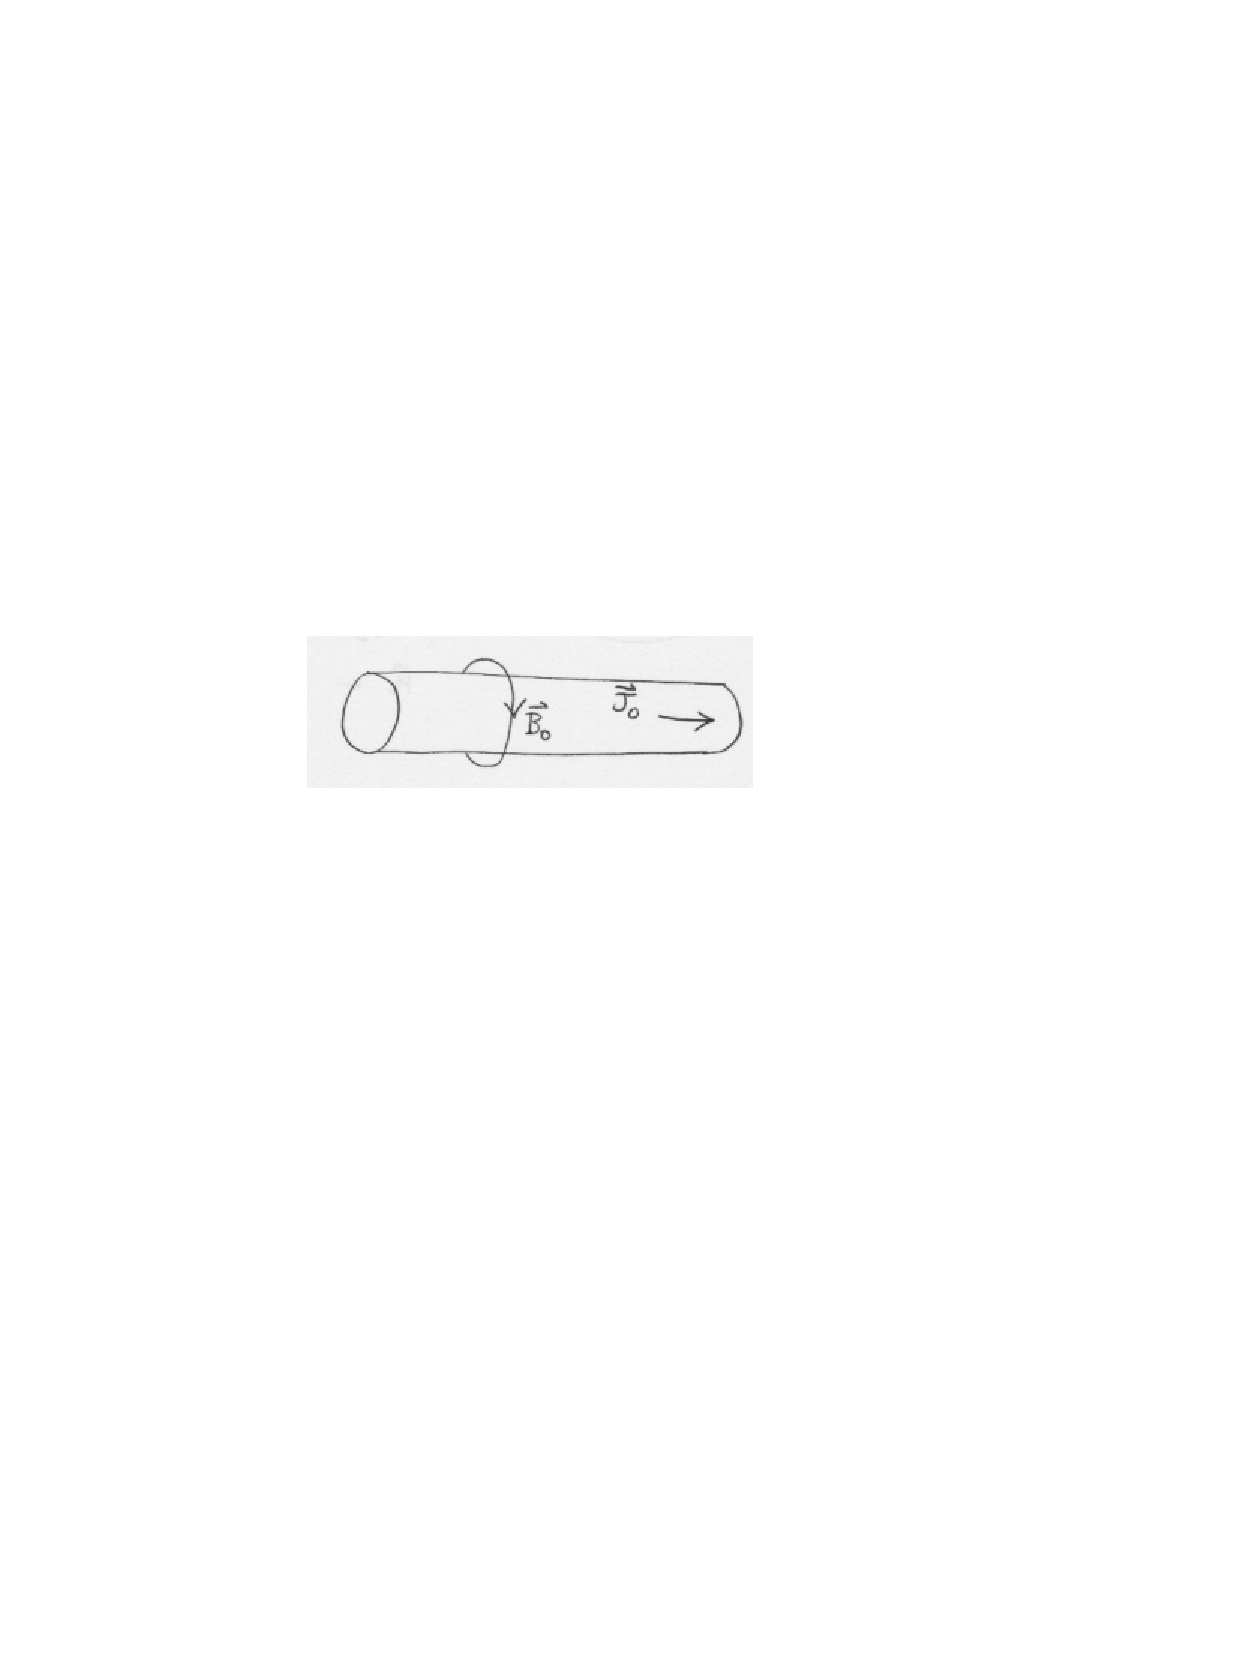
\includegraphics[width=0.3\textwidth]{figures/mhd_instability.pdf}
		\label{fig:zPinch}
		}
		\subfigure[]{%
		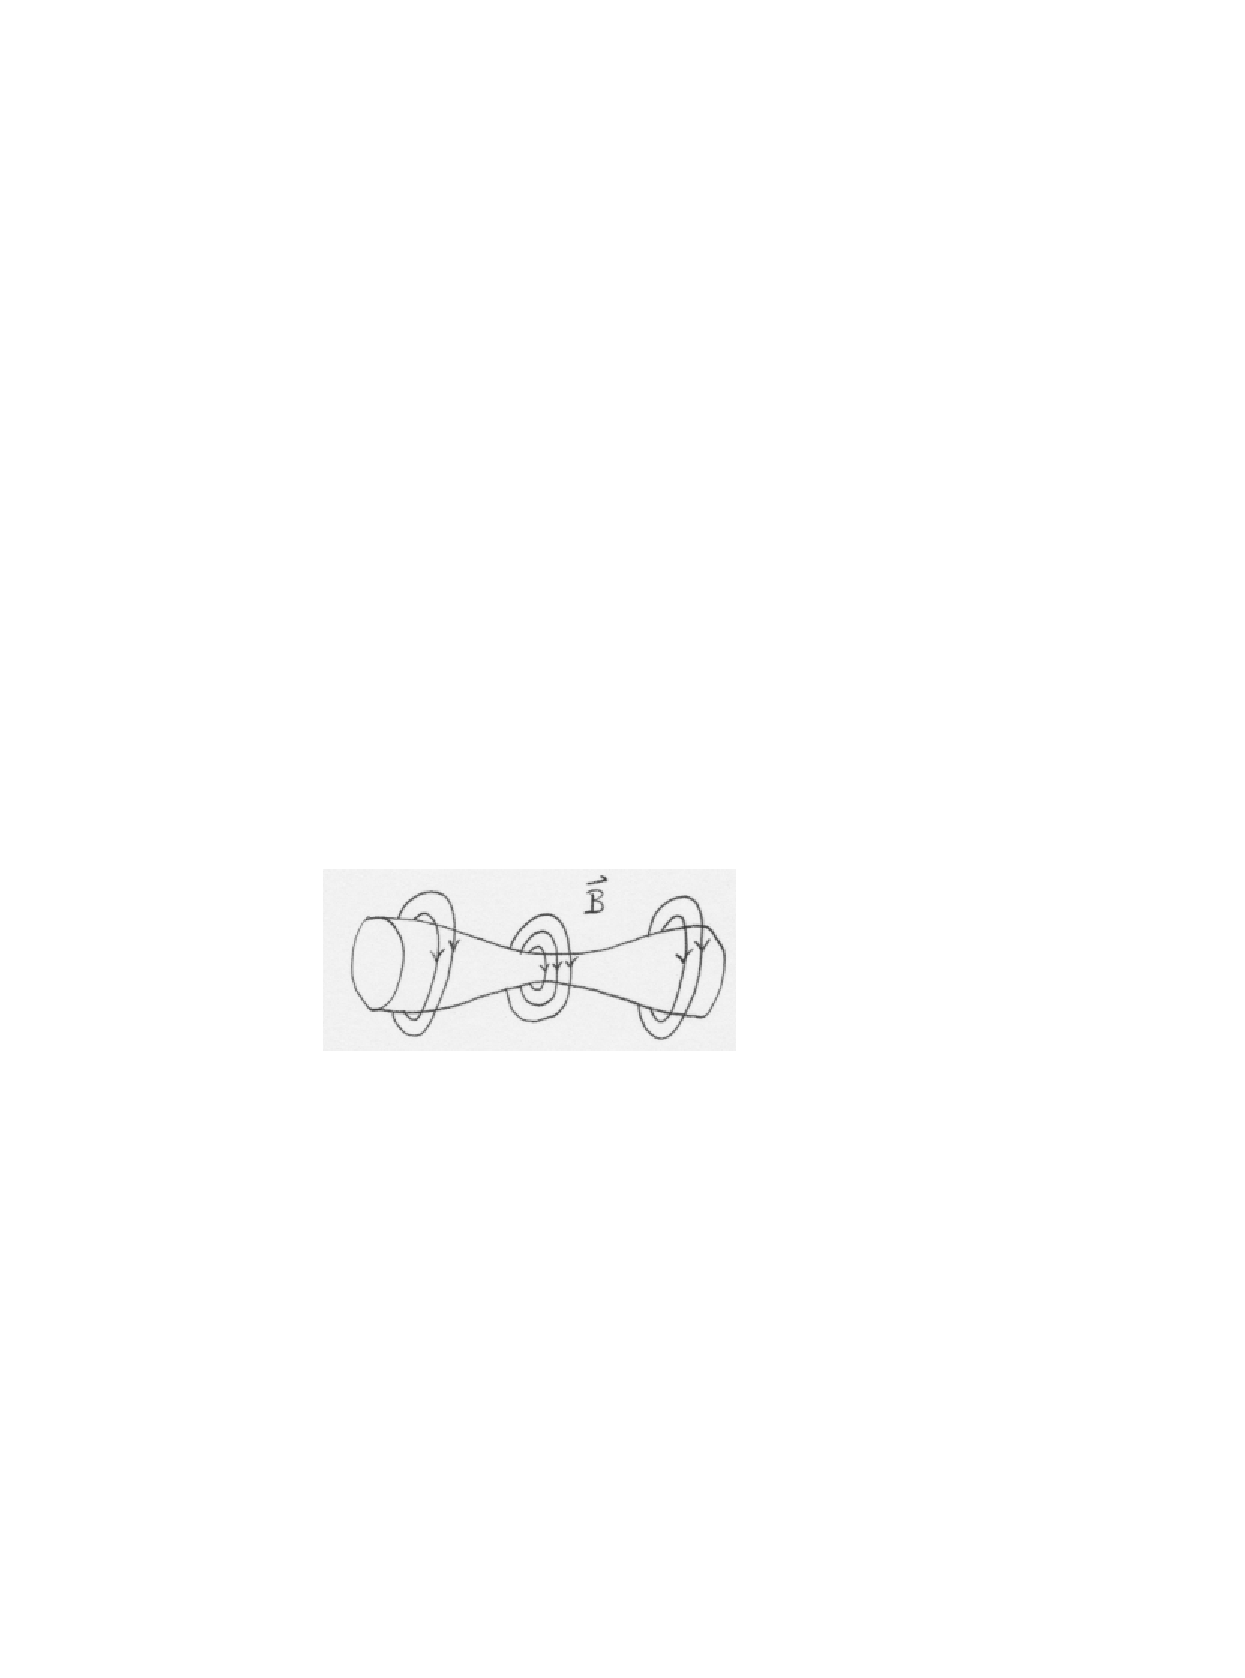
\includegraphics[width=0.3\textwidth]{figures/mhd_instability_sausage.pdf}
		\label{fig:sausage}
		}
		\subfigure[]{%
		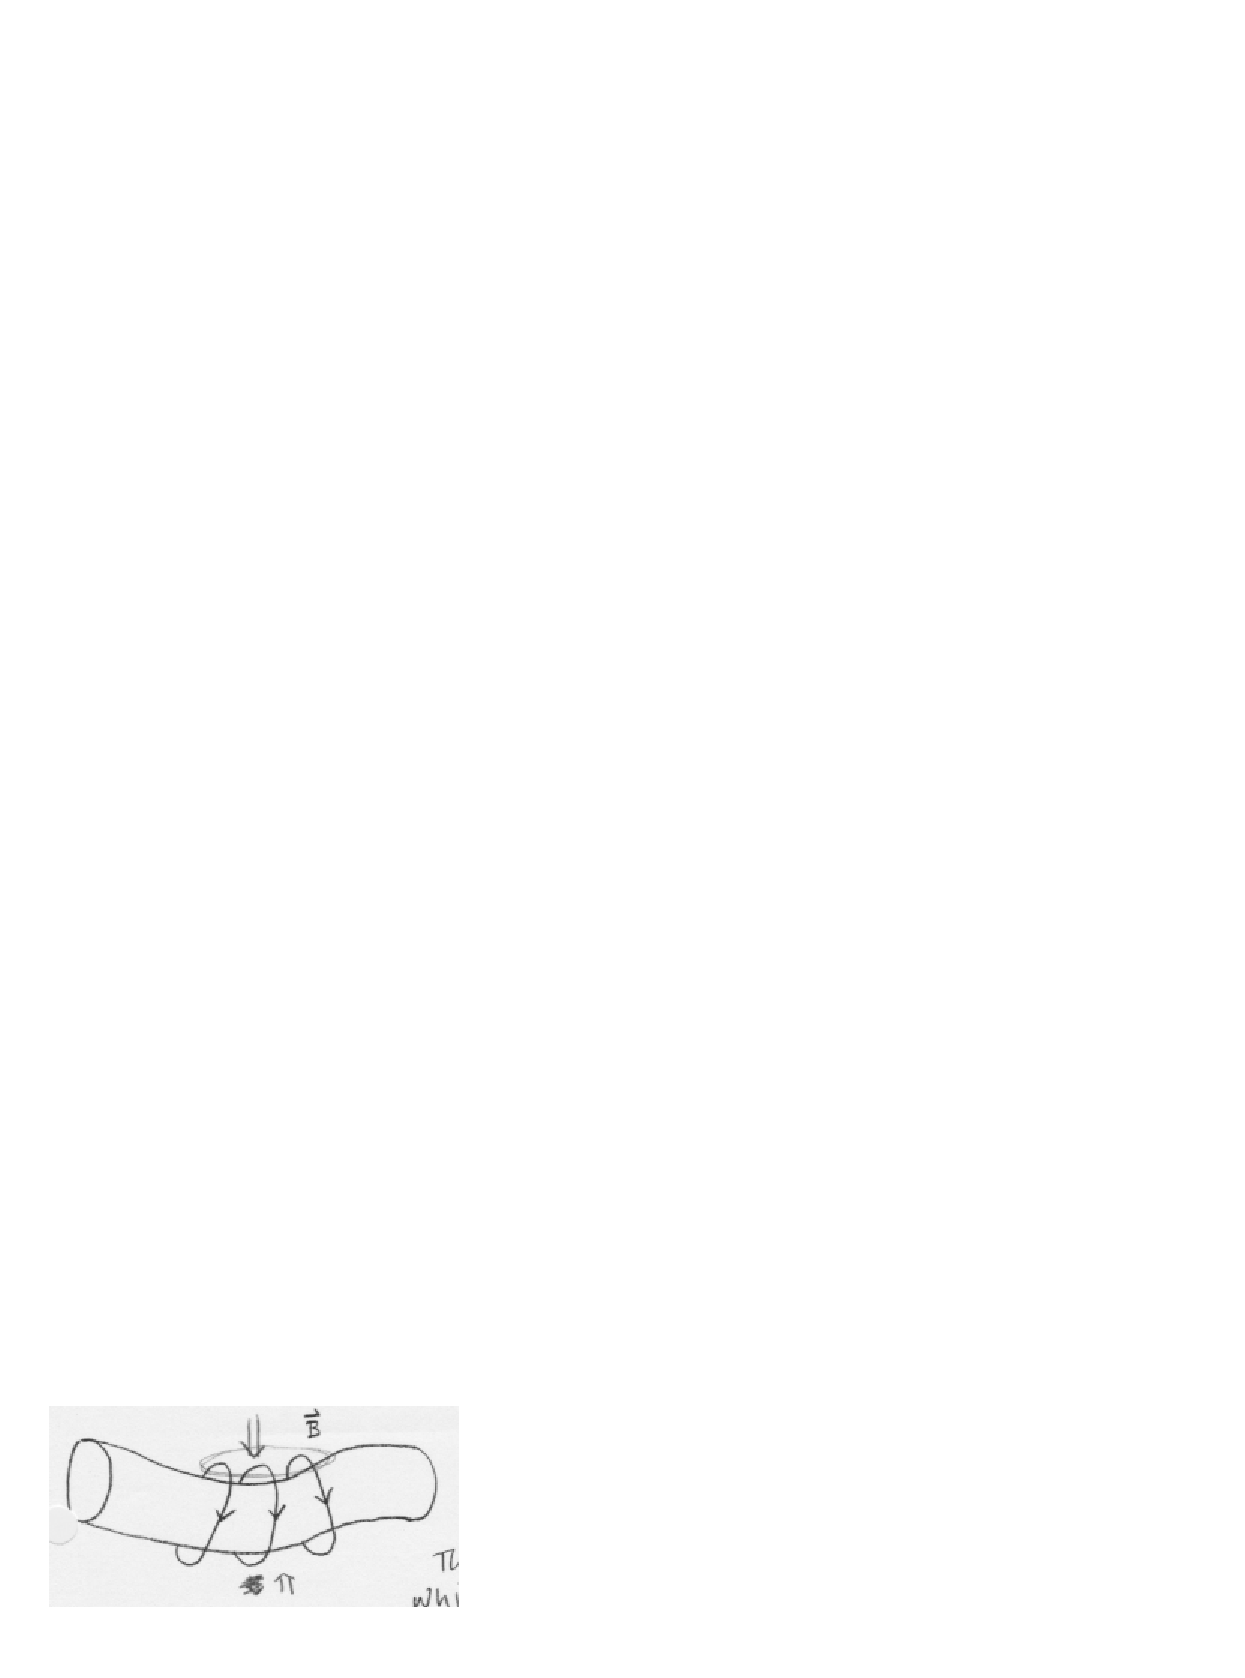
\includegraphics[width=0.3\textwidth]{figures/mhd_instability_kink.pdf}
		\label{fig:kink}
		}
		\caption{Cylindrical column of plasma that is \ref{fig:sausage} squeezed locally and potentially subject to a sausage mode and \ref{fig:kink} a bent tube potentially subject to the kink instability.}
		\label{fig:mhd_instabilities}
	\end{figure}

	To illustrate this, consider the cases in Fig. \ref{fig:mhd_instabilities}. First, in Fig. \ref{fig:zPinch} we have a cylindrical column of plasma with an axial current $J_z$ and an azimuthal magnetic field $\mathbf{B}_0$. Suppose the column is squeezed locally as Fig. \ref{fig:sausage}. Because the current through the column is uniform, the current density near the ``neck'' increases, giving a greater inward magnetic field tension. This tends to enhance the neck and the plasma can pinch off. This is called the \textit{sausage instability}.

	Now suppose the column is bent as in Fig. \ref{fig:kink}. The lines of azimuthal $\mathbf{B}$ are closer together above the column and farther apart below, leading to greater magnetic tension downward. This tends to enhance the bend in the column which can lead to an instability, usually referred to as the \textit{kink instability}. Note that both of these instabilities are $\nabla p_0 (=\mathbf{J}_0\times\mathbf{B}_0)$ instabilities.

	\subsection{Shocks}

	\subsection{Force and motion in MHD}
	The MHD momentum equation, using Amp\'ere's law to substitute for $\mathbf{j}$, can be written as,
	\begin{equation}
		\rho\frac{d\mathbf{v}}{dt} = \frac{4\pi}{c}(\nabla\times\mathbf{B})\times\mathbf{B} - \nabla p.
	\end{equation}
	Using vector identities, this can be rewritten as,
	\begin{equation}
		\rho\frac{d\mathbf{v}}{dt} = -\nabla\left(p + \frac{B^2}{8\pi/c}\right) + \frac{c}{4\pi}(\mathbf{B}\cdot\nabla)\mathbf{B}.
	\end{equation}
	From this expression, we can see how the presence of a magnetic field in a conducting fluid can set the fluid in motion. Using the fact that $\mathbf{B}=B\hat{b}$, where $\hat{b}$ is the unit vector in the local direction of the magnetic field, and $\partial\hat{b}/\partial s=\hat{n}/R$, where $\hat{n}$ is the unit vector normal to the magnetic field and $R$ is the local radius of curvature, this equation can be written,
	\begin{equation}
		\rho\frac{dv}{dt} = -\nabla p - \nabla_{\perp}\left(\frac{B^2}{8\pi/c}\right) + \frac{1}{R}\left(\frac{B^2}{4\pi/c}\right)\hat{n},
	\end{equation}
	where $\nabla_{\perp}\equiv\nabla - \hat{b}\partial/\partial s$, a gradient operator acting only in the direction perpendicular to the field. From this equation, it can be seen that the magnetic field exerts two types of forces on the fluid, neither of them parallel to the direction of the field. The second term on the right hand side represents a magnetic pressure term that acts to drive the fluid away fom regions of high magnetic field strength. The third term on the right hand side accelerates the fluid along $\hat{n}$ towards the center of curvature of the field line. This force acts to straighten the field line, reducing its curvature. Thus, this force describes a \textit{tension} in magnetic field lines. 

	Additionally, it should be noted that the time evolution of the field $\mathbf{B}$ following the fluid element is determined only by the initial value of $\mathbf{B}$ and the local stress tensor of the fluid element. The value of the field in neighbouring fluid elements is \textit{not} relevant. This holds for an incompressible fluid, $\nabla\cdot\mathbf{v}=0$. Relaxing this situation, this statement holds when changing $\mathbf{B}\to\mathbf{B}/\rho$. 

\section{Magnetic Reconnection}
See \cite{priest_magnetic_2000}

	\subsection{Basic features}
	Briefly, magnetic reconnection is the topological restructuring of the magnetic field as it relaxes from a stressed to equilibrium state. It is thought to be a dominant process in many astrophysical environments, including accretion disks and solar flares, as well as the Earth's magnetosphere. The basic underlying mechanism is as follows. When two oppositely-directed field lines are brought together in a conducting fluid, a tangential discontinuity develops between them, with current-carrying plasma squeezed into this area of discontinuity.

	Because these field lines are ``frozen'' into the plasma, a large magnetic gradient develops at the discontinuity called the diffusion region. In this region, because of the large magnetic field gradients, the resistivity becomes very high, allowing field lines to diffuse through the plasma, reconnect, and relax to a topologically different, but more energetically favorable state. As the field lines reconnect and are pushed out of the diffusion region, they accelerate and heat the plasma. Reconnection is thus a non-ideal process as it allows for the conversion of stored magnetic energy to kinetic and thermal energy via dissipation.

	\subsection{MHD models}
	The first complete theory of reconnection was proposed by \citet{sweet_neutral_1958} and \citet{parker_sweets_1957,parker_solar-flare_1963}, now commonly known as the Sweet-Parker mechanism. In the Sweet-Parker model, two anti-parallel field lines are carried into a diffusion region of length $2L$ and width $2\ell$ (where $L>\ell$) at velocity $v_i=\eta/\ell$, where $\eta$ is the magnetic diffusivity. Using Maxwell's equations and the mass and momentum conservation equations from MHD, the inflow velocity, or reconnection rate, can be written as,
	\begin{equation}
		v_i = \frac{v_{Ai}}{\sqrt{R_{mi}}},
	\end{equation}
	where $R_{mi}\equiv Lv_{Ai}/\eta$ is the magnetic Reynolds number. The problem with the Sweet-Parker mechanism, however, is that it predicts reconnection rates far too slow to properly account for observed energy release timescales in flare plasmas.

	In an attempt to remedy these slow reconnection rates, \citet{petschek_magnetic_1964} proposed that magnetoacoustic shocks could provide an additional acceleration into the diffusion region. This combined with a smaller diffusion region shortened the reconnection timescale. While it was initially believed that the Petschek mechanism solved the problem of fast reconnection, increasingly detailed observations and numerical simulations have shown that reconnection is a far more subtle mechanism than initially thought.

\section{Kinetic Description of Plasma}
We now move away from a fluid description of a plasma and instead treat the plasma as a collection of particles, each with positions $\mathbf{x}_i$ and velocities $\mathbf{v}_i$, where $i=1\ldots N$, with $N$ being the total number of particles. In this way, we can consider $N_{0s}$ particles of species $s$ moving through a six-dimensional phase space $(\mathbf{x},\mathbf{v})$. Thus, the \textit{phase space density} for this system can be expressed as,
\begin{equation}
	N_s(\mathbf{x},\mathbf{v},t) = \sum_{i=1}^{N_{0s}}\delta(\mathbf{x}-\mathbf{X}_{is}(t))\delta(\mathbf{v} - \mathbf{V}_{is}(t)),
\end{equation}
where $\mathbf{X}_{is}(t),\mathbf{V}_{is}(t)$ are the position and velocity of particle $i$ with species $s$ at time $t$. This is often called the Klimontovich density. These particles and fields satisfy the microscopic Newton-Lorentz and Maxwell equations. Using this and the definition of $N_s$, we can describe the time evolution of this phase space density using the Klimontovich equation,
\begin{equation}
	\frac{\partial}{\partial t}N_s + \mathbf{v}\cdot\nabla N_s + \frac{q_s}{m_s}\left(\mathbf{E}_m + \frac{1}{c}\mathbf{v}\times\mathbf{B}_m\right)\cdot\nabla_vN_s = 0.
\end{equation}
This equation is physically equivalent to the Newton-Lorentz equation and when written in conservative form can be interpreted as a statement of particle number conservation. It can also be shown that, along a particle trajectory, the Klimontovich density of species $s$ is constant, or way may say that it is \textit{incompressible}.

	\subsection{Vlasov theory}

	While the Klimontovich equation is exact, it is not very useful because in practice it cannot be solved. In fact, a quick calculation will show that it takes the age of the universe to find $N_s$ for any significant number of particles. Instead, define a phase space distribution that is an ensemble average (i.e. an average over many identically prepared systems with varying microscopic initial conditions) such that,
	\begin{equation}
		f_s(\mathbf{x},\mathbf{v},t) \equiv \langle N_s(\mathbf{x},\mathbf{v},t)\rangle.
	\end{equation}
	Writing $N,\mathbf{E}_m,\mathbf{B}_m$ in the form $\phi_m = \phi + \delta\phi$, plugging into the Klimontovich density and taking an ensemble average, 
	\begin{equation}
		\frac{\partial}{\partial t}f_s + \mathbf{v}\cdot\nabla_xf_s + \frac{q_s}{m_s}\left(\mathbf{E} + \frac{1}{c}\mathbf{v}\times\mathbf{B}\right)\cdot\nabla_vf_s = -\frac{q_s}{m_s}\left\langle\left(\delta\mathbf{E}_m + \frac{1}{c}\mathbf{v}\times\delta\mathbf{B}_m\right)\cdot\nabla_v\delta N_s\right\rangle.
	\end{equation}
	This is the \textit{plasma kinetic equation}. The left hand side contains smmoth continuous ensemble averaged quantities. The right hand side is an ensemble average of spikey, discrete single-particle quantities. It can be shown that the ratio of the right hand side to the left hand side is proportional to $\Lambda^{-1}$ such that RHS$\ll$LHS when $\Lambda\gg1$, where $\Lambda$, the plasma parameter, represents the number of particles in the Debye cube. Physically, the RHS represents effects of EM interactions between individual particles (i.e. collisions). In the limit of $\Lambda\to\infty$, we may neglect the RHS such that,
	\begin{empheq}[box=\widefbox]{align}
		\frac{\partial}{\partial t}f_s + \mathbf{v}\cdot\nabla_xf_s + \frac{q_s}{m_s}\left(\mathbf{E} + \frac{1}{c}\mathbf{v}\times\mathbf{B}\right)\cdot\nabla_vf_s = 0,
	\end{empheq}
	the Vlasov equation. If we combine this equation with the Maxwell equations where the charge and current are given by
	\begin{align}
		\rho =& \sum_sq_s\int\mathrm{d}^3vf_s, \\
		\mathbf{j} =& \sum_sq_s\int\mathrm{d}^3v\mathbf{v}f_s,
	\end{align}
	we get the Vlasov-Maxwell equations. The Vlasov equation does \textit{not} include effects due to binary Coulomb collisions though collisions can be introduced by adding a term on the right hand side of the form $\partial f_s/\partial t|_C$. The Vlasove equation is a fluid equation in 6D phase space that includes more information about the velocity distributions of the particles (e.g. as compared to MHD). The $\mathbf{v}$ here is not a bulk flow velocity, but rather a phase space coordinate independent of $\mathbf{x}$ and $t$. 

	\subsection{Landau damping}

	The Vlasov equation can be linearized by expressing the phase space distribution as $f(\mathbf{x},\mathbf{v},t) = f_0(\mathbf{v}) + \delta f(\mathbf{x},\mathbf{v},t)$. Using this and our definition of the charge density $\rho$, the Gauss equation can be written
	\begin{equation}
		\nabla\cdot\delta\mathbf{E} = -4\pi e\int\mathrm{d}^3v\delta f.
	\end{equation}
	Additionally, assuming only electrostatic perturbations (i.e. $\delta\mathbf{B}=0$), we can write down a linearized Vlasov equation of the form
	\begin{equation}
		\frac{\partial}{\partial t}\delta f + \mathbf{v}\cdot\nabla_x\delta f + -\frac{e}{m_e}\delta\mathbf{E}\cdot\nabla_v\delta f_0 = 0.
	\end{equation}
	Together, these two equations provide a closed set of integro-differential equations for electrostatic electron plasma waves in an unmagnetized Vlasov plasma (for given $f_0$).

	We can now use plane-wave solutions (as we did in the waves section) to solve for $\delta f$ and plug into our modified Gauss equation. Choosing $\mathbf{k}=k\hat{z}$, we find that
	\begin{equation}
	\epsilon(\mathbf{k},\omega)\equiv 1 +\frac{4\pi e^2}{mk}\int\mathrm{d}^3v\frac{\partial f_0/\partial v_z}{\omega - kv_z} = 0.
	\end{equation}
	This is the dielectric function and is a dispersion relation (i.e. it relates $\omega$ and $k$).

	Notice that the denominator can go to zero if $\omega=kv_z$. This corresponds to a resonant wave-particle interaction. Imagine that there is a test particle with speed $v_z=\omega/k$ and a large number of particles with velocity close to (but not equal to) the wave phase velocity. Now, let the number of particles with $v_z\lesssim\omega/k$ be $n_{-}$ and the number of particles with $v_z\gtrsim\omega/k$ be $n_{+}$. If $n_-\neq n_+$, there is a net force on the $n_-+n_+$ particles. \textit{This net force can transfer energy between the wave and the particles}. This happens because of particles with velocities near the phase speed of the wave. In particular, if $n_->n_+$, the wave can be dampled by the particles with speeds near $\omega/k$. This damping is the collective, collisionless phenomenon known as \textit{Landau damping}.

	The general approach to obtaining a result is to first Taylor expand $\epsilon(k,\omega)$ about $\omega=\omega_r$, $\epsilon(k,\omega_r+i\omega_i)$. By assuming weak damping/growth, we assume $|\omega_i|\ll|\omega_r|$ and $|\epsilon_i|\ll|\epsilon_r|$. Thus, to first order, 
	\begin{equation}
	\epsilon(k,\omega) \simeq \epsilon_r(k,\omega_r) + i\epsilon_i(k,\omega_r) + i\omega_i\frac{\partial\epsilon_r}{\partial\omega}\big|_{\omega=\omega_r}.
	\end{equation}
	By setting the real and imaginary parts equal, we get that
	\begin{align}
	\epsilon_r(k,\omega_r) = 0, \\
	\omega_i = -\frac{\epsilon_i(k,\omega_r)}{\partial\epsilon_r(k,\omega_r)/\partial\omega_r}.
	\end{align}
	To integrate around the pole at $\omega/k$, we introduce collisions through the Krook model which lifts the path off of the real axis by $i\nu_C$. Solving for $\omega_i$ assuming $f_0$ is a Maxwellian, we find that
	\begin{equation}
	\frac{\omega_i}{\omega_{pe}} = -\frac{\sqrt{8\pi}}{k^3\lambda_D^3}\exp{\left(\frac{-2}{k^2\lambda_D^2}\right)}.
	\end{equation}
	Note that $\omega_i<0$, corresponding to Landau damping. $\omega_i$ follows from the negative slope of $f_0$: there are more particles moving slightly slower than the wave, thus taking energy from the wave, causing it to be damped. 

	\subsection{Basic kinetic instabilities}
	\subsection{Fokker-Planck equation and binary coulomb collisions}
